% !TEX root = ../PDE4ML.tex

\section{Dynamic Optimal Transport}
\index{dynamic!optimal transport}% strictindex
\label{sec-dynamic-optimal-transport}
\label{sec-wasserstein-flows}

Optimal transport becomes especially useful for machine learning once distances between probability laws are written as actions of moving mass. This section is synchronized with the full OT4ML manuscript and keeps the material needed later in the survey: continuity equations, the Benamou--Brenier formula, path-space viewpoints, and generalized dynamic distances that later generate PDE flows.\index{continuity equation}% strictindex
\index{Benamou-Brenier formula}% strictindex
\index{generalized dynamic Wasserstein distance}% strictindex

\subsection{Evolutions over the Space of Measures}
\index{measure!evolution}% strictindex

We start with the continuity equation because it is the common language for particles, densities and weak measure evolutions. It also makes precise which velocity fields actually move mass.
\index{velocity field}% strictindex
\index{continuity equation}% strictindex

\paragraph{Lagrangian and Eulerian descriptions.}
\index{Lagrangian!description}% strictindex
\index{Eulerian!description}% strictindex

We consider the evolution $t \mapsto \alpha_t \in \Pp(\RR^d)$. Such an evolution can be described in a ``Lagrangian'' way as the advection of particles along a (time-dependent) vector field $v_t(x)$ in $\RR^d$. At the particle level, this advection is governed by
\index{time-dependent vector field}% strictindex
\begin{equation}
    \frac{\d x(t)}{\d t} = v_t(x(t)), \label{eq:lagrangian-advection}
\end{equation}
and we write $T_t$ for the associated flow map, so that $T_t(x(0))=x(t)$. The advected measure is then $\alpha_t = (T_t)_\sharp \alpha_0$. For discrete measures, $\alpha_t = \frac{1}{n} \sum_{i=1}^n \delta_{x_i(t)}$, meaning each $x_i(t)$ solves \eqref{eq:lagrangian-advection}.
\index{flow!map}% strictindex

In the Eulerian description, the same motion is written directly on the evolving measure: the particle ODE becomes the PDE
\index{particle ODE}% strictindex
\index{Eulerian!description}% strictindex
\begin{equation}
    \frac{\partial \alpha_t}{\partial t} + \diverg(v_t \alpha_t) = 0. \label{eq:eulerian-advection}
\end{equation}
This PDE is often referred to as the advection equation, the continuity equation, or Liouville's equation when operating over a phase space. It is only a classical PDE when $\alpha_t$ has a smooth density. For general measures, and in particular for empirical measures, it is understood in the weak sense: for any smooth test function $(t,x)\mapsto\varphi(t,x)$ compactly supported in time,
\index{empirical!measure}% strictindex
\index{continuity equation}% strictindex
\begin{equation}\label{eq:eulerian-advection-weak}
	\int_0^1\!\int_{\RR^d}
	\left(\partial_t\varphi(t,x)+\dotp{v_t(x)}{\nabla_x\varphi(t,x)}\right)
	\d\alpha_t(x)\d t
	=
	0.
\end{equation}
This equation is obtained from~\eqref{eq:eulerian-advection} by integration by parts. Hence, for smooth positive densities, the classical and weak formulations are equivalent; the weak formulation is useful because it still makes sense for discrete measures whose particles evolve according to~\eqref{eq:lagrangian-advection}.

\begin{prop}[Lagrangian flows solve the continuity equation]\label{prop-lagrangian-flow-continuity}
\index{Lagrangian!flow}% strictindex
\index{continuity equation}% strictindex
	Consider a smooth flow $T_t:\RR^d\to\RR^d$ and define $\alpha_t=(T_t)_\sharp\alpha_0$. Define the Eulerian velocity field by
\index{velocity field}% strictindex
\index{Eulerian!velocity}% strictindex
	\[
		v_t(T_t(y))=\partial_t T_t(y).
	\]
	Then $(\alpha_t,v_t)$ solves the continuity equation in the weak sense~\eqref{eq:eulerian-advection-weak}.
	In particular, if $\alpha_0=\frac1n\sum_i\delta_{x_i(0)}$ is empirical, then $\alpha_t=\frac1n\sum_i\delta_{x_i(t)}$ is empirical as well, with particle velocities $\dot x_i(t)=v_t(x_i(t))$.
\end{prop}

\begin{proof}
	Let $\varphi(t,x)$ be a smooth test function vanishing at $t=0$ and $t=1$. Since $\alpha_t=(T_t)_\sharp\alpha_0$,
	\[
		\frac{\d}{\d t}\int \varphi(t,x)\d\alpha_t(x)
		=
		\frac{\d}{\d t}\int \varphi(t,T_t(y))\d\alpha_0(y).
	\]
	The chain rule gives
	\[
		\frac{\d}{\d t}\int \varphi(t,T_t(y))\d\alpha_0(y)
		=
		\int
		\left(
			\partial_t\varphi(t,T_t(y))
			+\dotp{\nabla_x\varphi(t,T_t(y))}{\partial_t T_t(y)}
		\right)
		\d\alpha_0(y).
	\]
	Using the definition of $v_t$ and the push-forward relation, this equals
\index{push-forward}% strictindex
	\[
		\int
		\left(
			\partial_t\varphi(t,x)+\dotp{\nabla_x\varphi(t,x)}{v_t(x)}
		\right)
		\d\alpha_t(x).
	\]
	Integrating in time and using the boundary values of $\varphi$ gives~\eqref{eq:eulerian-advection-weak}.
\end{proof}

\paragraph{From measure evolutions to vector fields.}
\index{measure!evolution}% strictindex

For a given evolution $(\alpha_t)_t$, there are typically infinitely many velocity fields $v_t$ satisfying
\index{velocity field}% strictindex
\begin{equation}\label{eq:inverse-flow}
	\partial_t\alpha_t+\diverg(\alpha_t v_t)=0.
\end{equation}
This non-uniqueness comes from the kernel of the weighted divergence. The linear space of vector fields that leave a measure $\alpha$ invariant is
\[
	\Hh_\alpha=\enscond{v}{\diverg(\alpha v)=0}.
\]
It is usually non-trivial: for instance, if $\alpha$ is an isotropic Gaussian, $\Hh_\alpha$ contains rotational vector fields generated by anti-symmetric matrices.

\paragraph{Dacorogna--Moser inversion.}
\index{Dacorogna-Moser inversion}% strictindex
\index{Dacorogna-Moser construction}% strictindex

Reconstructing particles from an observed density evolution is therefore ill-posed. A simple choice, introduced by Dacorogna and Moser~\cite{DacorognaMoser1990}, is to impose that the flux $\alpha_t v_t$ is a gradient field, leading formally to
\index{flux}% strictindex
\begin{equation}\label{eq:dacorogna-moser}
	v_t=-\frac{1}{\alpha_t}\nabla\Delta^{-1}(\partial_t\alpha_t),
\end{equation}
with suitable boundary conditions, for instance vanishing at infinity. This formula is useful conceptually but delicate when $\alpha_t$ vanishes, and it does not generally produce a gradient velocity field.
\index{velocity field}% strictindex
\index{gradient!velocity}% strictindex

The classical Dacorogna--Moser construction uses the linear density path. If $\alpha_i=\rho_i\,\d x$ are smooth positive densities with the same total mass on a bounded domain $\Omega$, set
\[
	\alpha_t=(1-t)\alpha_0+t\alpha_1=\rho_t\,\d x,
	\qquad
	\rho_t=(1-t)\rho_0+t\rho_1.
\]
Choose a time-independent flux $w$ satisfying
\[
	\diverg w=\rho_0-\rho_1,
	\qquad
	w\cdot n=0\quad\hbox{on }\partial\Omega,
\]
for instance $w=-\nabla\phi$ with $\Delta\phi=\rho_1-\rho_0$ and Neumann boundary condition. Then
\[
	v_t=\frac{w}{\rho_t}
\]
satisfies $\partial_t\rho_t+\diverg(\rho_t v_t)=0$. The flow
$\partial_t T_t=v_t\circ T_t$, $T_0=\Id$, therefore transports
$\rho_0\d x$ onto $\rho_t\d x$, and $T_1$ solves the prescribed-Jacobian problem
$\rho_1(T_1(x))\det(\nabla T_1(x))=\rho_0(x)$.

\paragraph{Least-square inversion and gradient structure.}
\index{least-square!inversion}% strictindex
\index{gradient!structure}% strictindex

A more robust choice, used implicitly in flow matching, optimal transport and Wasserstein gradient flows, is to select among all admissible velocities the one with smallest kinetic energy:
\index{Wasserstein gradient}% strictindex
\index{gradient!flow}% strictindex
\index{Wasserstein!gradient flow}% strictindex
\index{flow matching}% strictindex
\begin{equation}\label{eq:least-square-field}
	\umin{v}
	\frac12\int_0^1\!\int_{\RR^d}\norm{v_t(x)}^2\,\d\alpha_t(x)\d t
	\quad
	\text{subject to}
	\quad
	\partial_t\alpha_t+\diverg(\alpha_t v_t)=0.
\end{equation}

\begin{prop}[Least-square velocities are gradients]\label{prop-least-square-gradient-velocity}
\index{least-square!velocity}% strictindex
\index{gradient!velocity}% strictindex
	Assume that $\alpha_t=\rho_t\,\d x$ is a smooth positive density curve and that boundary terms vanish. The minimizer of~\eqref{eq:least-square-field}, if it exists, is a gradient field
	\[
		v_t=\nabla\phi_t,
	\]
	where $\phi_t$, unique up to an additive constant, solves the weighted Poisson equation
\index{weighted!Poisson equation}% strictindex
	\begin{equation}\label{eq:least-square-field-explicit}
		-\diverg(\rho_t\nabla\phi_t)=\partial_t\rho_t,
		\qquad
		v_t=-\nabla\Delta_{\alpha_t}^{-1}(\partial_t\alpha_t),
		\quad
		\Delta_{\alpha_t}\phi=\diverg(\alpha_t\nabla\phi).
	\end{equation}
\end{prop}

\begin{proof}
	Introduce a Lagrange multiplier $\phi_t$ for the continuity equation. The constrained problem has the formal saddle formulation
\index{continuity equation}% strictindex
	\[
		\umin{v}\umax{\phi}
		\int_0^1
		\left[
			\frac12\int_{\RR^d}\norm{v_t(x)}^2\,\d\alpha_t(x)
			+\int_{\RR^d}\phi_t(x)\big(\diverg(\alpha_t v_t)(x)+\partial_t\alpha_t(x)\big)\d x
		\right]\d t.
	\]
	Integrating by parts in the divergence term gives, for each $t$,
	\[
		\int \left(\frac12\norm{v_t}^2-\dotp{\nabla\phi_t}{v_t}\right)\d\alpha_t
		+
		\int \phi_t\,\partial_t\alpha_t .
	\]
	The pointwise minimizer in $v_t$ is therefore $v_t=\nabla\phi_t$. Substituting this into the constraint $\partial_t\rho_t+\diverg(\rho_t v_t)=0$ gives the weighted Poisson equation in~\eqref{eq:least-square-field-explicit}. The inverse notation is just a shorthand for solving this equation on zero-mean right-hand sides, modulo additive constants.
\index{zero mean}% strictindex
\index{weighted!Poisson equation}% strictindex
\end{proof}

In general this inversion is still computationally demanding, but special choices of $(\alpha_t)_t$ lead to simpler formulas; this is the mechanism exploited later by flow matching in Section~\ref{sec-generative-flow-matching}.
\index{flow matching}% strictindex

\subsection{Benamou--Brenier dynamic formulation of OT}
\index{Benamou-Brenier}% strictindex
\index{Benamou-Brenier formulation}% strictindex
\index{Benamou-Brenier formula}% strictindex
\label{sec-benamou-brenier-dynamic}

The dynamic formulation identifies $\Wass_2$ with the kinetic energy of the cheapest continuity-equation path. It is the point where OT becomes a least-action principle.
\index{continuity equation}% strictindex
\index{dynamic!formulation}% strictindex

\paragraph{Benamou--Brenier formulation.}

Instead of assuming that a whole curve $(\alpha_t)_{t\in[0,1]}$ is prescribed, one only fixes its endpoints $\alpha_0$ and $\alpha_1$ and minimizes the least-square energy~\eqref{eq:least-square-field}. The theorem of Benamou and Brenier states that this geodesic energy is exactly the squared Wasserstein distance~\cite{benamou2000computational}.
\index{Wasserstein!distance}% strictindex

\begin{thm}[Benamou--Brenier]\label{thm-benamou-brenier}
\index{Benamou-Brenier}% strictindex
	For probability measures $\alpha_0,\alpha_1\in\Pp_2(\RR^d)$,
\index{probability measure}% strictindex
	\begin{equation}\label{eq:benamou-brenier}
	\Wass_2^2(\alpha_0,\alpha_1)
	=
	\inf_{(\alpha_t,v_t)}
	\int_0^1\!\int_{\RR^d}\norm{v_t(x)}^2\,\d\alpha_t(x)\d t,
	\end{equation}
	where the infimum is over $(\alpha_t,v_t)$ solving $\partial_t\alpha_t+\nabla\!\cdot(\alpha_t v_t)=0$ with $\alpha_{t=0}=\alpha_0$ and $\alpha_{t=1}=\alpha_1$. If $\alpha_0$ has a density and $T$ is the optimal Monge map $T_\sharp\alpha_0=\alpha_1$, the minimizer is
\index{Monge!problem}% strictindex
	\begin{equation}\label{eq:static-to-dynamic}
		\alpha_t=((1-t)\Id+tT)_\sharp\alpha_0,
		\qquad
		v_t\big((1-t)x+tT(x)\big)=T(x)-x.
	\end{equation}
\end{thm}

\begin{proof}
	For the inequality ``dynamic $\leq$ static'', assume first that a Monge map $T$ exists and define $(\alpha_t,v_t)$ by~\eqref{eq:static-to-dynamic}. Since the Lagrangian velocity $T(x)-x$ is independent of $t$,
\index{Monge!problem}% strictindex
	\[
		\int_0^1\!\int\norm{v_t}^2\,\d\alpha_t\d t
		=
		\int\norm{T(x)-x}^2\,\d\alpha_0(x),
	\]
	so the dynamic cost is no larger than the static Monge cost. Without a Monge map, the same construction is made with an optimal coupling $\pi$: sample $(X,Y)\sim\pi$ and move along the straight path $\gamma_{X,Y}(t)=(1-t)X+tY$. This path measure has action $\int\norm{x-y}^2\d\pi(x,y)$; projecting path velocities onto their conditional mean at time $t$ gives an admissible Eulerian velocity with no larger action, so the dynamic value is no larger than the Kantorovich value.
\index{dynamic value}% strictindex
\index{optimal coupling}% strictindex
\index{Eulerian!velocity}% strictindex
\index{path measure}% strictindex

	Conversely, for a smooth deterministic path, take the flow $T_t$ defined by $\dot T_t=v_t\circ T_t$ and $T_0=\Id$. Then $\alpha_t=(T_t)_\sharp\alpha_0$ and $(T_1)_\sharp\alpha_0=\alpha_1$. Jensen's inequality gives
\index{Jensen inequality}% strictindex
	\[
		\norm{T_1(x)-x}^2
		\leq
		\int_0^1\norm{v_t(T_t(x))}^2\d t.
	\]
	After integration with respect to $\alpha_0$, the Monge cost is bounded above by the dynamic action. For general finite-energy solutions of the continuity equation, the superposition principle lifts the curve to a probability measure on absolutely continuous paths; applying Jensen's inequality pathwise gives a coupling of the endpoints whose quadratic cost is no larger than the action. Thus the Kantorovich value is bounded above by the dynamic value.
\index{dynamic value}% strictindex
\index{absolutely continuous path}% strictindex
\index{dynamic action}% strictindex
\index{superposition principle}% strictindex
\index{Jensen inequality}% strictindex
\index{probability measure}% strictindex
\index{continuity equation}% strictindex
\index{quadratic cost}% strictindex
\end{proof}

\paragraph{Convex moment-based reformulation.}
\index{momentum formulation}% strictindex

Although~\eqref{eq:benamou-brenier} is not jointly convex in $(\alpha_t,v_t)$, it becomes convex after replacing velocities by the momentum measure $m_t=v_t\alpha_t$ and using the perspective action. In the absolutely continuous case $\alpha_t=\rho_t\,\d x$ and $m_t(x)=\rho_t(x)v_t(x)$, this reads
\index{perspective function}% strictindex
\index{momentum}% strictindex
\index{Benamou-Brenier}% strictindex
\begin{equation}\label{eq:benamou-brenier-convex}
	\Wass_2^2(\alpha_0,\alpha_1)
	=
	\inf_{\substack{\partial_t\rho_t+\diverg m_t=0\\
	\rho_{t=0}\d x=\alpha_0,\ \rho_{t=1}\d x=\alpha_1}}
	\int_0^1\!\int_{\RR^d}
	\frac{\norm{m_t(x)}^2}{\rho_t(x)}\,\d x\,\d t,
	\end{equation}
with the usual convention that the integrand is $0$ when $(\rho_t,m_t)=(0,0)$ and $+\infty$ when $\rho_t=0$ but $m_t\neq0$. For singular endpoints or curves, the same statement is interpreted with vector-valued momentum measures and the corresponding recession convention. This convex reformulation enables geodesic interpolation by convex optimization once the domain is discretized.
\index{recession convention}% strictindex
\index{momentum}% strictindex

\paragraph{Dual Hamilton--Jacobi formulation.}
\index{Hamilton-Jacobi equation}% strictindex
\index{Benamou-Brenier dual}% strictindex

The momentum formulation also has a useful dual. It turns the least-action problem into a Hamilton--Jacobi subsolution inequality for a scalar potential, with equality on the part of space-time actually visited by the optimal curve. This is the dual dynamic formulation already present in the original Benamou--Brenier perspective~\cite{benamou2000computational}; see also the standard accounts~\cite{Villani03,SantambrogioBook}. The constants below follow the convention of~\eqref{eq:benamou-brenier-convex}, where the kinetic energy has no factor $1/2$.
\index{perspective function}% strictindex

\begin{prop}[Dual Benamou--Brenier problem]\label{prop-benamou-brenier-dual}
	Assume, for simplicity, that the densities are smooth, compactly supported, and that boundary terms vanish. Then the convex dynamic value~\eqref{eq:benamou-brenier-convex} has the dual formulation
	\begin{equation}\label{eq:benamou-brenier-dual}
		\Wass_2^2(\alpha_0,\alpha_1)
		=
		\sup_{\phi}
		\enscond{
		\int_{\RR^d}\phi_1\,\d\alpha_1
		-
		\int_{\RR^d}\phi_0\,\d\alpha_0
		}{
		\partial_t\phi_t+\frac14\norm{\nabla\phi_t}^2\leq 0
		},
	\end{equation}
	where the supremum is over smooth test potentials $\phi:[0,1]\times\RR^d\to\RR$. In the general metric-measure statement, the same formula is understood after relaxation: $\phi$ is a Hamilton--Jacobi subsolution, for instance in the viscosity sense, and finite-dimensional discretizations follow directly from Fenchel--Rockafellar duality.
\index{Hamilton-Jacobi equation}% strictindex

	If $(\rho,m)$ and $\phi$ are smooth primal and dual optimizers, then
	\begin{equation}\label{eq:bb-primal-dual-relation}
		m_t=\frac{\rho_t}{2}\nabla\phi_t,
		\qquad
		\partial_t\phi_t+\frac14\norm{\nabla\phi_t}^2=0
		\quad\text{on }\{\rho_t>0\}.
	\end{equation}
	Equivalently, the optimal Eulerian velocity is $v_t=m_t/\rho_t=\nabla\phi_t/2$.
\index{Eulerian!velocity}% strictindex
\end{prop}

\begin{proof}
	Let $(\rho,m)$ satisfy the continuity equation and let $\phi$ be smooth. Multiplying the constraint by $\phi$ and integrating by parts gives
\index{continuity equation}% strictindex
	\[
		\int_{\RR^d}\phi_1\,\d\alpha_1
		-
		\int_{\RR^d}\phi_0\,\d\alpha_0
		=
		\int_0^1\!\int_{\RR^d}
		\left(\rho_t\,\partial_t\phi_t+\dotp{m_t}{\nabla\phi_t}\right)\d x\d t .
	\]
	If $\partial_t\phi_t+\norm{\nabla\phi_t}^2/4\leq0$, Young's inequality yields, pointwise,
	\[
		\rho\,\partial_t\phi+\dotp{m}{\nabla\phi}
		\leq
		-\frac{\rho}{4}\norm{\nabla\phi}^2+\dotp{m}{\nabla\phi}
		\leq
		\frac{\norm m^2}{\rho},
	\]
	with the same perspective convention when $\rho=0$. Hence the dual objective of every feasible $\phi$ is no larger than the action of every feasible primal pair.
\index{perspective function}% strictindex

	Conversely, introduce $\phi$ as a Lagrange multiplier for $\partial_t\rho+\diverg m=0$. After integration by parts, and up to the fixed endpoint contribution in~\eqref{eq:benamou-brenier-dual}, the pointwise minimization over $(\rho,m)$ contains
	\[
		\frac{\norm m^2}{\rho}-\rho\,\partial_t\phi-\dotp{m}{\nabla\phi}.
	\]
	For fixed $\rho>0$, its minimum over $m$ is attained at $m=\rho\nabla\phi/2$ and equals $-\rho(\partial_t\phi+\norm{\nabla\phi}^2/4)$. The infimum over $\rho\geq0$ is finite exactly when the Hamilton--Jacobi inequality holds, in which case the pointwise infimum is $0$. Fenchel--Rockafellar duality then gives no duality gap. Equality in the two pointwise inequalities gives~\eqref{eq:bb-primal-dual-relation}.
\index{Hamilton-Jacobi equation}% strictindex
\index{Fenchel-Rockafellar duality}% strictindex
\index{perspective function}% strictindex
\end{proof}

This also recovers the static Kantorovich inequality from a dynamic principle. If $\gamma$ is any smooth curve with $\gamma(0)=x$ and $\gamma(1)=y$, then
\[
	\frac{\d}{\d t}\phi_t(\gamma(t))
	=
	\partial_t\phi_t(\gamma(t))+\dotp{\nabla\phi_t(\gamma(t))}{\dot\gamma(t)}
	\leq
	\norm{\dot\gamma(t)}^2,
\]
where the last inequality uses $\partial_t\phi+\norm{\nabla\phi}^2/4\leq0$ and Young's inequality. Integrating and minimizing over curves gives
\[
	\phi_1(y)-\phi_0(x)\leq\norm{x-y}^2.
\]
Thus $(\phi_0,\phi_1)$ is a feasible static Kantorovich dual pair for the quadratic cost. At optimality the inequality is saturated on the endpoint pairs connected by the primal characteristics, which is the Eulerian version of complementary slackness.
\index{Kantorovich!dual}% strictindex
\index{complementary slackness}% strictindex

\begin{figure}[ht]
\centering
\begin{tabular}{@{}ccc@{}}
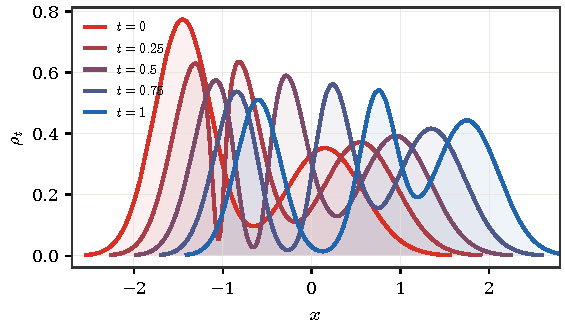
\includegraphics[width=.31\linewidth]{figures/dynamic-benamou-brenier-duality/density.pdf} &
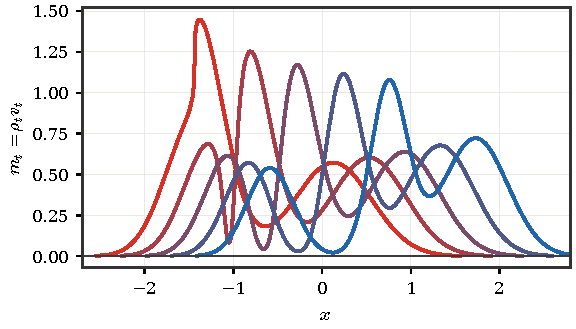
\includegraphics[width=.31\linewidth]{figures/dynamic-benamou-brenier-duality/momentum.pdf} &
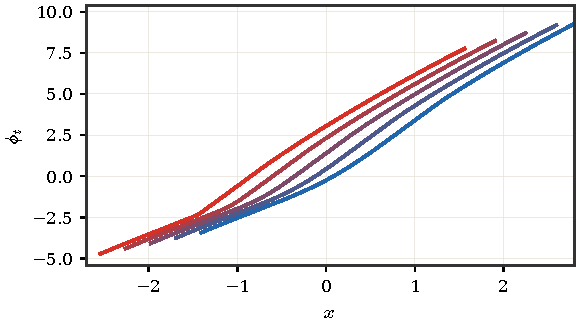
\includegraphics[width=.31\linewidth]{figures/dynamic-benamou-brenier-duality/dual-potential.pdf}
\\[-.1em]
\small density $\rho_t$ &
\small momentum $m_t$ &
\small dual potential $\phi_t$
\end{tabular}
\caption{\emph{One-dimensional Benamou--Brenier primal and dual solutions.} The endpoints are Gaussian mixtures and the solution is computed from monotone quantile interpolation. The left and middle panels show the primal density and momentum $m_t=\rho_t v_t$. The right panel shows the dual Hamilton--Jacobi potential, normalized up to an additive constant. Along the active transported mass, the notebook checks the primal--dual identities $m_t=\rho_t\partial_x\phi_t/2$ and $\partial_t\phi_t+|\partial_x\phi_t|^2/4=0$.}
\index{Hamilton-Jacobi equation}% strictindex
\index{momentum}% strictindex
\label{fig:dynamic-benamou-brenier-duality}
\end{figure}

\paragraph{Proximal splitting.}
\index{proximal!splitting}% strictindex
\index{Douglas-Rachford splitting}% strictindex

The convex momentum formulation also explains the original Benamou--Brenier solver. Papadakis, Peyr\'e and Oudet~\cite{FPapPeyOud13} showed that, after discretization, the ALG2 scheme is a Douglas--Rachford splitting, equivalently ADMM on the Fenchel--Rockafellar dual. Suppressing discretization indices, write $U=(\rho,m)$ and introduce the perspective integrand
\index{perspective function}% strictindex
\[
	J(\rho,m)=
	\begin{cases}
		\norm{m}^2/\rho, & \rho>0,\\
		0, & (\rho,m)=(0,0),\\
		+\infty, & \text{otherwise}.
	\end{cases}
\]
Let
\[
	\mathcal F(U)=\int_0^1\!\int_{\RR^d}J(\rho_t(x),m_t(x))\,\d x\,\d t,
	\qquad
	\mathcal C=\enscond{(\rho,m)}{\partial_t\rho+\diverg m=0,\ \rho_0\d x=\alpha_0,\ \rho_1\d x=\alpha_1},
\]
and let $\mathcal G=\iota_{\mathcal C}$ be the indicator of this affine continuity constraint. The convex Benamou--Brenier problem is therefore
\[
	\min_U\; \mathcal F(U)+\mathcal G(U).
\]
On the resulting Hilbert space of unknowns, or formally for an $L^2$-type product structure, the two proximal operators are
\index{proximal!operator}% strictindex
\[
	\prox_{\tau\mathcal F}(\bar U)
	=
	\argmin_U
	\frac12\norm{U-\bar U}_{\mathsf H}^2+\tau\mathcal F(U),
	\qquad
	\prox_{\tau\mathcal G}(\bar U)
	=
	\argmin_{U\in\mathcal C}
	\frac12\norm{U-\bar U}_{\mathsf H}^2 .
\]
For the standard product metric, the first map is local in $(t,x)$: it is the proximal operator of the convex perspective $J$. The second map is the orthogonal projection onto the affine set defined by the divergence equation and endpoint constraints. Douglas--Rachford then alternates these two simple operations:
\index{proximal!operator}% strictindex
\index{Douglas-Rachford algorithm}% strictindex
\[
	\begin{aligned}
		U^{k+1} &= \prox_{\tau\mathcal F}(Z^k),\\
		\widetilde U^{k+1} &= \prox_{\tau\mathcal G}(2U^{k+1}-Z^k),\\
		Z^{k+1} &= Z^k+\widetilde U^{k+1}-U^{k+1}.
	\end{aligned}
\]
Equivalently one may swap the roles of $\mathcal F$ and $\mathcal G$. At convergence, the two shadow sequences $U^k$ and $\widetilde U^k$ agree and give a minimizer of the convex dynamic problem. This viewpoint is useful because it separates the nonlinear but pointwise perspective proximal step from the global but linear projection onto the continuity equation~\cite{FPapPeyOud13,Eckstein1992}.
\index{perspective function}% strictindex
\index{continuity equation}% strictindex
\index{Fenchel-Rockafellar duality}% strictindex
\index{ADMM}% strictindex

\begin{alg}[Douglas--Rachford for dynamic Benamou--Brenier]\label{alg:benamou-brenier-douglas-rachford}
\index{Douglas-Rachford splitting}% strictindex
\textbf{Input:} Functionals $\mathcal F,\mathcal G=\iota_{\mathcal C}$, proximal parameter $\tau>0$, initial field $Z^0$.

\textbf{Output:} Discrete density-momentum field $U^\star$.

\textbf{For} $k=0,1,\ldots$ \textbf{do}:
\begin{algblock}
\(U^{k+1}=\prox_{\tau\mathcal F}(Z^k).\)

\textbf{Project} reflected point:
\(\widetilde U^{k+1} = \prox_{\tau\mathcal G}(2U^{k+1}-Z^k) = \Proj_{\mathcal C}(2U^{k+1}-Z^k).\)

\textbf{Update}
\(Z^{k+1}=Z^k+\widetilde U^{k+1}-U^{k+1}.\)

\textbf{If} $\norm{U^{k+1}-\widetilde U^{k+1}}\leq\mathrm{tol}$ \textbf{then}:
\begin{algblock}
\textbf{Return} $U^{k+1}$.
\end{algblock}
\end{algblock}
\end{alg}

\begin{figure}[ht]
\centering
\newcommand{\bbgeodesicpanelheight}{.155\linewidth}
\begin{tabular}{@{}cc@{}}

\includegraphics[height=\bbgeodesicpanelheight]{figures/dynamic-benamou-brenier-geodesic/density-sequence.pdf} &
\index{Benamou-Brenier}% strictindex
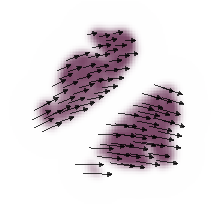
\includegraphics[height=\bbgeodesicpanelheight]{figures/dynamic-benamou-brenier-geodesic/midpoint-velocities.pdf}
\\[-.1em]
\small density sequence &
\small midpoint velocities
\end{tabular}
\caption{\emph{Benamou--Brenier geodesic between two sampled silhouettes.} A discrete quadratic OT plan between finely subsampled cat and two-disks point clouds induces the McCann interpolation $Z_t=(1-t)X+tY$, which is the Lagrangian realization of the least-action solution. The left panel renders local color images of the smaller-bandwidth kernel-smoothed densities with enough padding to include the full silhouettes. The right panel overlays shortened velocity arrows centered at evenly subsampled midpoint particles $Z_{1/2}$; each displayed arrow runs in data coordinates from a source-side tail to a target-side head along the matched characteristic direction $Y-X$, but is not drawn as the full endpoint segment from $X$ to $Y$.}
\index{McCann interpolation}% strictindex
\label{fig:dynamic-benamou-brenier-geodesic}
\end{figure}

\paragraph{Path-space formulation.}\label{rem-bb-path-space}
\index{path-space formulation}% strictindex
	Let $\Ss=C([0,1];\RR^d)$ be the space of continuous paths endowed with the uniform topology. For $t\in[0,1]$ define the evaluation map
	\[
		P_t:\Ss\to\RR^d,
		\qquad
		P_t(\gamma)=\gamma(t).
	\]
	The Benamou--Brenier cost admits the equivalent formulation
\index{Benamou-Brenier}% strictindex
	\[
		\Wass_2^2(\alpha_0,\alpha_1)
		=
		\inf_{M\in\Pp(\Ss)}
		\enscond{
			\int_{\Ss}\!\int_0^1\norm{\dot\gamma(t)}^2\d t\,\d M(\gamma)
		}{
			(P_0)_\sharp M=\alpha_0,\ (P_1)_\sharp M=\alpha_1
		}.
	\]
	If $\alpha_0$ has a density, the minimizer $M^*$ is unique. Its time marginals reproduce the optimal curve: $\alpha_t=(P_t)_\sharp M^*$ for all $t$. Furthermore, for a.e. $t$, denoting $Q_t(\gamma)=\dot\gamma(t)$ on absolutely continuous paths, the conditional law of the velocity is deterministic:
\index{absolutely continuous path}% strictindex
\index{conditional law}% strictindex
	\[
		(P_t,Q_t)_\sharp M^*(\d x,\d q)
		=
		\alpha_t(\d x)\delta_{v_t^*(x)}(\d q),
	\]
	where $v_t^*$ is the optimal velocity field in the Benamou--Brenier formulation. Hence $M^*$ concentrates on straight-line geodesics and, for a.e. $t$, assigns exactly one direction at $\alpha_t$-a.e. spatial point.
\index{Benamou-Brenier}% strictindex
\index{velocity field}% strictindex
\index{Benamou-Brenier formulation}% strictindex

\subsection{Generalized Dynamic Wasserstein Distances}
\index{dynamic!formulation}% strictindex
\label{sec-bb-extensions}
\label{sec-generalized-dynamic-wasserstein-distances}

The quadratic Benamou--Brenier formula is only one instance of a broader fixed-mass dynamic language. The goal of this section is to define a large family of geodesic-like distances on spaces of probability measures by modifying the action minimized in the Benamou--Brenier formula. The objects introduced here are metric: they specify admissible curves, tangent variables and path energies. All descent constructions are postponed to Section~\ref{sec-generalized-dynamic-wasserstein-flows}, where these distances are used to generate gradient-flow PDE models; the reaction--transport case, where mass may vary, is separated in Section~\ref{sec-unbalanced-ot}.
\index{Wasserstein!distance}% strictindex
\index{perspective function}% strictindex

\paragraph{Path actions.}
\index{path action}% strictindex
The common starting point is an instantaneous cost for moving a measure with a prescribed Eulerian velocity. Integrating this cost along continuity-equation curves produces the associated endpoint geometry.

In the mass-preserving Euclidean setting, the basic input is an instantaneous action $\mathbb A(\alpha,w)$, where \(\alpha\) is the current measure and \(w\) is an admissible velocity representative. When this action is normalized as a squared infinitesimal speed, it generates the length-space value
\begin{equation}\label{eq-generalized-action-length-distance}
	\mathsf D_{\mathbb A}^2(\alpha_0,\alpha_1)
	=
	\inf_{\alpha_t,v_t}
	\left\{
	\int_0^1 \mathbb A(\alpha_t,v_t)\,\d t
	:
	\partial_t\alpha_t+
	\diverg(\alpha_t v_t)=0,\
	\alpha_{t=0}=\alpha_0,\
		\alpha_{t=1}=\alpha_1
	\right\}.
\end{equation}
Equivalently, one may quotient by velocity fields that induce the same first-order variation of the measure. The formula~\eqref{eq-generalized-action-length-distance} should be read as a dynamic definition of the distance, not as a property automatically satisfied by an arbitrary discrepancy. Some standard distances, such as \(\Wass_p\), are first written with a \(p\)-homogeneous action and then squared by taking a constant-speed parametrization; this normalization is made explicit below. Different choices of \(\mathbb A\) change the resulting geometry; Section~\ref{sec-generalized-dynamic-wasserstein-flows} later reuses these choices when dynamics are introduced.

\paragraph{Quadratic, or Riemannian, tangent actions.}
\index{local tangent action}% strictindex
\index{squared local action}% strictindex
\index{local action}% strictindex
\index{tangent action}% strictindex
\index{length space}% strictindex
\index{geodesic distance}% strictindex
\index{quadratic action}% strictindex
\index{Onsager operator}% strictindex
\index{Riemannian metric}% strictindex
\index{tangent norm}% strictindex
\index{quadratic tangent norm}% strictindex
A particularly transparent case occurs when \(w\mapsto\mathbb A(\alpha,w)\) is quadratic. For simplicity, take admissible velocities in \(L^2(\alpha;\RR^d)\); in some applications this Hilbert space is replaced by a closed subspace encoding additional constraints. If the polarization of \(\mathbb A\) is represented by a positive self-adjoint operator
\(Q_\alpha:L^2(\alpha;\RR^d)\to L^2(\alpha;\RR^d)\),
\[
	\mathbb A(\alpha;w,z)
	=
	\left\langle Q_\alpha w,z\right\rangle_{L^2(\alpha)},
	\qquad
	\mathbb A(\alpha,w)=\left\langle Q_\alpha w,w\right\rangle_{L^2(\alpha)},
\]
and if this quadratic form is nondegenerate after quotienting velocities that induce the same measure variation, then the least-action distance generated by this tensor is
\begin{equation}\label{eq-general-quadratic-tangent-action}
	\mathsf D_Q^2(\alpha_0,\alpha_1)
	=
	\mathsf D_{\mathbb A}^2(\alpha_0,\alpha_1)
	=
	\inf_{\substack{\partial_t\alpha_t+\diverg(\alpha_t v_t)=0\\
	\alpha_{t=0}=\alpha_0,\ \alpha_{t=1}=\alpha_1}}
	\int_0^1
	\left\langle Q_{\alpha_t}v_t,v_t\right\rangle_{L^2(\alpha_t)}
	\d t .
\end{equation}
The usual $\Wass_2$ geometry corresponds to $Q_\alpha=\Id$ in this simplified notation. Thus \(Q_\alpha\) records how the chosen geometry deforms the Euclidean \(L^2(\alpha)\) tangent norm: no deformation for \(\Wass_2\), and a nontrivial tensor for generalized Riemannian geometries. In Section~\ref{sec-generalized-dynamic-wasserstein-flows}, the same tensor is reused as a preconditioner for metric descent.
\index{Hilbertian tangent norm}% strictindex
\index{Riemannian tensor}% strictindex
\index{Riemannian metric}% strictindex

\paragraph{Local velocity actions.}
\index{action density}% strictindex
\index{momentum variable}% strictindex
\index{momentum formulation}% strictindex
Many dynamic distances are local with respect to a reference measure $\lambda$. Write $\alpha=a\lambda$. A velocity action is specified by a pointwise integrand
\[
	A:[0,+\infty)\times\RR^d\to[0,+\infty],
	\qquad
	(a,w)\mapsto A(a,w),
\]
where $a\in\RR_+$ is a density value and $w\in\RR^d$ is a velocity value, and defines
\begin{equation}\label{eq-local-velocity-action}
	\mathbb A(\alpha,w)
	=
	\int A\left(\frac{\d\alpha}{\d\lambda}(x),w(x)\right)\d\lambda(x).
\end{equation}
For a fixed reference $\lambda$, this covers density-dependent mobilities and congestion constraints. If, in addition, $A$ is positively $1$-homogeneous in its first variable, $A(\eta a,w)=\eta A(a,w)$ for $\eta\geq0$, then the same formula is intrinsic: replacing $\lambda$ by another dominating measure gives the same value. The usual Benamou--Brenier action is the model case
\begin{equation}\label{eq-bb-velocity-action}
	A_2(a,w)=a\norm{w}^2,
	\qquad
	\mathbb A(\alpha,w)=\int\norm{w}^2\d\alpha .
\end{equation}
Here \(a=\d\alpha/\d\lambda\) is the density of transported mass and \(w\) is the Eulerian velocity. The factor \(a\) says that moving twice as much mass with the same velocity costs twice as much.

\paragraph{Homogeneous momentum actions.}\label{rem-generalized-bb}
\index{Benamou-Brenier}% strictindex
\index{Benamou-Brenier distance}% strictindex
\index{convex action density}% strictindex
The same action can be written in momentum variables, and this is the form in which convexity and metric properties are easiest to read. Set $\omega=\alpha w$, so that $\omega$ is a vector-valued measure. When the local description is written with the same reference $\lambda$, so that $\alpha=a\lambda$ and $\omega=m\lambda$, the pointwise momentum perspective is
\begin{equation}\label{eq-general-momentum-perspective}
	J_A(a,m)
	\eqdef
	\begin{cases}
	A(a,m/a), & a>0,\\
	0, & a=0\ \text{and}\ m=0,\\
	+\infty, & a=0\ \text{and}\ m\neq0,
	\end{cases}
\end{equation}
and the measure action relative to $\lambda$ is
\begin{equation}\label{eq-general-measure-momentum-action}
	\mathbb J_{A,\lambda}(\alpha,\omega)
	\eqdef
	\int
	J_A\!\left(
		\frac{\d\alpha}{\d\lambda},
		\frac{\d\omega}{\d\lambda}
	\right)\d\lambda,
\end{equation}
with value \(+\infty\) if \(\alpha\) or the total variation \(|\omega|\) is not absolutely continuous with respect to \(\lambda\). This zero-density convention is the lower-semicontinuous one for the superlinear actions used below; other growths use the corresponding recession extension. If $A$ is positively $1$-homogeneous in $a$, then $J_A$ is jointly $1$-homogeneous: $J_A(\eta a,\eta m)=\eta J_A(a,m)$. In that intrinsic case the value of \(\mathbb J_{A,\lambda}\) is independent of the dominating reference measure, and we write simply \(\mathbb J_A\). For $A_2(a,w)=a\norm{w}^2$, one recovers the quadratic perspective
\[
	J_2(a,m)=\frac{\norm m^2}{a},
\]
which is the integrand used in the convex Benamou--Brenier formulation~\eqref{eq:benamou-brenier-convex}. In this case \(\omega=\alpha w\); if \(\alpha=\rho\d x\) and \(\omega=m\d x\), then \(m=\rho w\), and \(J_2(\rho,m)=\rho\norm w^2\).
\index{perspective function}% strictindex
\index{quadratic perspective}% strictindex

\begin{prop}[Concave mobilities give convex momentum actions]\label{prop-momentum-perspective-convexity}
\index{perspective function}% strictindex
\index{convex action density}% strictindex
\index{momentum formulation}% strictindex
	Let \(I\subset[0,+\infty)\) be a convex interval, let \(\theta:I\to[0,+\infty)\) be concave, and let \(L:\RR^d\to[0,+\infty]\) be convex with \(L(0)=0\). Define, on the set where \(\theta(a)>0\),
	\begin{equation}\label{eq-concave-mobility-perspective}
		J_{\theta,L}(a,m)
		\eqdef
		\theta(a)L\!\left(\frac{m}{\theta(a)}\right),
		\qquad
		A_{\theta,L}(a,w)
		\eqdef
		J_{\theta,L}(a,aw)
		=
		\theta(a)L\!\left(\frac{aw}{\theta(a)}\right),
	\end{equation}
	and extend \(J_{\theta,L}\) to the boundary by lower semicontinuity. Then \(J_{\theta,L}\) is convex in \((a,m)\). In particular, this single construction contains
	\[
		A(a,w)=aL(w)
		\quad\text{by taking }\theta(a)=a,
	\]
	and the concave-mobility quadratic action
	\[
		A(a,w)=\frac{a^2\norm{w}^2}{\theta(a)}
		\quad\text{by taking }L(u)=\norm u^2.
	\]
\end{prop}

\begin{proof}
	The perspective \(P(s,m)=sL(m/s)\) of a convex function is convex on \(s>0\). Since \(L(0)=0\), it is also nonincreasing in the scalar \(s\) for fixed \(m\): if \(s_2\geq s_1>0\), then
	\[
		L(m/s_2)
		=
		L\big((s_1/s_2)(m/s_1)\big)
		\leq
		(s_1/s_2)L(m/s_1),
	\]
	hence \(P(s_2,m)\leq P(s_1,m)\). Let \(a_\zeta=(1-\zeta)a_0+\zeta a_1\) and \(m_\zeta=(1-\zeta)m_0+\zeta m_1\). By concavity of \(\theta\),
	\[
		\theta(a_\zeta)
		\geq
		(1-\zeta)\theta(a_0)+\zeta\theta(a_1).
	\]
	Using the monotonicity in \(s\), and then the convexity of \(P\), gives
	\[
		J_{\theta,L}(a_\zeta,m_\zeta)
		=
		P(\theta(a_\zeta),m_\zeta)
		\leq
		P((1-\zeta)\theta(a_0)+\zeta\theta(a_1),m_\zeta)
		\leq
		(1-\zeta)J_{\theta,L}(a_0,m_0)+\zeta J_{\theta,L}(a_1,m_1).
	\]
	The boundary cases follow by the chosen lower-semicontinuous extension.
	\end{proof}

The next proposition isolates the additional assumptions under which the momentum formulation generated by \(A\) defines a genuine path metric rather than only a variational principle.
\index{dynamic!formulation}% strictindex
\index{lower semicontinuous relaxation}% strictindex

\begin{prop}[Homogeneous dynamic actions define distances]\label{prop-homogeneous-dynamic-action-distance}
\index{dynamic!distance}% strictindex
\index{homogeneous action}% strictindex
\index{finite-action component}% strictindex
	Fix a reference measure \(\lambda\), omitted from the notation only in the intrinsic case where \(\mathbb J_{A,\lambda}\) does not depend on \(\lambda\). Assume that the momentum perspective \(J_A\) defined in~\eqref{eq-general-momentum-perspective} is lower semicontinuous, convex in \((a,m)\), even in \(m\), and satisfies \(J_A(a,0)=0\). Assume moreover that for some \(r>1\)
	\[
			J_A(a,\xi m)=|\xi|^rJ_A(a,m)
			\qquad
			\text{for all admissible }a,\ \text{all }m,\ \text{and all }\xi\in\RR,
	\]
	and that \(J_A(a,m)=0\) if and only if \(m=0\). Equivalently, the evenness, homogeneity and nondegeneracy assumptions translate, away from zero density, into
	\[
		A(a,-w)=A(a,w),
		\qquad
		A(a,\xi w)=|\xi|^rA(a,w),
		\qquad
		A(a,w)=0 \Longleftrightarrow w=0
		\qquad (a>0).
	\]
	Define, on every fixed-mass class,
	\[
		\mathsf D_{A,\lambda}(\alpha_0,\alpha_1)
		\eqdef
		\inf_{\substack{\partial_t\alpha_t+\diverg\omega_t=0\\
		\alpha_{t=0}=\alpha_0,\ \alpha_{t=1}=\alpha_1}}
		\left(
		\int_0^1\mathbb J_{A,\lambda}(\alpha_t,\omega_t)\,\d t
		\right)^{1/r}.
	\]
	After the usual lower-semicontinuous relaxation assuming that zero-action values are attained, \(\mathsf D_{A,\lambda}\) is an extended distance on each finite-action component: it is symmetric, satisfies the triangle inequality, and \(\mathsf D_{A,\lambda}(\alpha_0,\alpha_1)=0\) only when \(\alpha_0=\alpha_1\). In the intrinsic case, we write \(\mathsf D_A\).
\end{prop}

\begin{proof}
	The constant curve \(\alpha_t=\alpha_0\), \(\omega_t=0\), gives \(\mathsf D_{A,\lambda}(\alpha_0,\alpha_0)=0\). Conversely, if \(\mathsf D_{A,\lambda}(\alpha_0,\alpha_1)=0\), the relaxed zero-action minimizer satisfies
	\[
		\int_0^1 \mathbb J_{A,\lambda}(\alpha_t,\omega_t)\,\d t=0.
	\]
	Since \(\mathbb J_{A,\lambda}\geq0\), this implies \(\omega_t=0\) for a.e. \(t\). The continuity equation then gives \(\partial_t\alpha_t=0\) in the sense of distributions, so \(\alpha_0=\alpha_1\).

	Symmetry follows by time reversal. If \((\alpha_t,\omega_t)_{t\in[0,1]}\) connects \(\alpha_0\) to \(\alpha_1\), then
	\[
		\widetilde\alpha_t=\alpha_{1-t},
		\qquad
		\widetilde\omega_t=-\omega_{1-t}
	\]
	connects \(\alpha_1\) to \(\alpha_0\), satisfies the same continuity equation, and has the same action because \(J_A\) is even in \(m\).

	It remains to prove the triangle inequality. Let \((\alpha^1,\omega^1)\) connect \(\alpha_0\) to \(\alpha_1\) with action \(E_1\), and let \((\alpha^2,\omega^2)\) connect \(\alpha_1\) to \(\alpha_2\) with action \(E_2\). For \(\tau\in(0,1)\), concatenate the two curves after the time changes \(s=t/\tau\) and \(s=(t-\tau)/(1-\tau)\):
	\[
		(\alpha_t,\omega_t)=
		\begin{cases}
			\bigl(\alpha^1_{t/\tau},\,\tau^{-1}\omega^1_{t/\tau}\bigr), & 0\leq t\leq \tau,\\[.2em]
			\bigl(\alpha^2_{(t-\tau)/(1-\tau)},\,(1-\tau)^{-1}\omega^2_{(t-\tau)/(1-\tau)}\bigr), & \tau\leq t\leq1.
		\end{cases}
	\]
	The rescaled curve is admissible from \(\alpha_0\) to \(\alpha_2\). By \(r\)-homogeneity in the momentum variable, its action is
	\[
		\tau^{1-r}E_1+(1-\tau)^{1-r}E_2.
	\]
	Writing \(X=E_1^{1/r}\) and \(Y=E_2^{1/r}\), the optimal allocation is \(\tau=X/(X+Y)\), with the evident limiting convention if \(X+Y=0\), and gives
	\[
		\inf_{\tau\in(0,1)}
		\left\{\tau^{1-r}E_1+(1-\tau)^{1-r}E_2\right\}
		=
		(X+Y)^r.
	\]
	Hence \(\mathsf D_{A,\lambda}(\alpha_0,\alpha_2)\leq E_1^{1/r}+E_2^{1/r}\). Taking \(E_1\) and \(E_2\) arbitrarily close to the two optimal action values yields
	\[
		\mathsf D_{A,\lambda}(\alpha_0,\alpha_2)
		\leq
		\mathsf D_{A,\lambda}(\alpha_0,\alpha_1)+\mathsf D_{A,\lambda}(\alpha_1,\alpha_2),
	\]
	with the usual extended-real convention when one of the distances is infinite.
\end{proof}

Without homogeneity or nondegeneracy, the same momentum action remains useful as a variational principle, but its \(r\)-th root need not define a distance.

\begin{example}[Wasserstein-\texorpdfstring{$p$}{p} action]
\index{Wasserstein-p action}% strictindex
	The usual $\Wass_p$ distances correspond to changing only the homogeneity of the Benamou--Brenier action. The case $p=2$ is the original formula~\cite{benamou2000computational}; for $1<p<+\infty$, the same dynamic viewpoint gives the standard description of absolutely continuous curves in Wasserstein spaces~\cite{ambrosio2006gradient,Villani03,SantambrogioBook}. The specific objects to insert in the general framework above are
	\[
		A_p(a,w)=a\norm{w}^p,
		\qquad
		J_p(a,m)=
		\begin{cases}
			\norm{m}^p/a^{p-1}, & a>0,\\
			0, & (a,m)=(0,0),\\
			+\infty, & a=0,\ m\neq 0,
		\end{cases}
	\]
	With \(A=A_p\), Proposition~\ref{prop-homogeneous-dynamic-action-distance} gives the usual identity \(\mathsf D_{A_p}=\Wass_p\). The corresponding squared length-space normalization is
	\[
		\mathbb A_p(\alpha,w)
		=
		\left(\int\norm{w}^p\d\alpha\right)^{2/p}.
	\]
	This is the squared version of the \(p\)-homogeneous action: minimizing \(\int_0^1\mathbb A_p(\alpha_t,v_t)\d t\) gives \(\Wass_p^2\) after constant-speed reparametrization. Thus \(A_p,J_p\) denote the local \(p\)-homogeneous velocity and momentum densities, whereas \(\mathbb A_p\) denotes the squared tangent action used in the length formulation. The endpoint $p=1$ can be treated separately: the perspective becomes \(J_1(a,m)=\norm m\), and the dynamic problem collapses to Beckmann's formulation of $\Wass_1$~\cite{Beckmann52}.
\index{Wasserstein!distance}% strictindex
\index{Beckmann!formulation}% strictindex
\end{example}

\paragraph{Concave-mobility actions.}
\index{concave mobility}% strictindex
\index{convex action density}% strictindex
\index{mobility!convexity mechanism}% strictindex
\index{mobility}% strictindex
One can instead keep a quadratic momentum action and change the mobility. Dolbeault, Nazaret and Savar\'e introduced this construction as a class of generalized transport distances adapted to nonlinear diffusion~\cite{dolbeault2009new}. Let \(I\subset[0,+\infty)\) be a convex interval and let \(\theta:I\to[0,+\infty)\) be concave. Define the extended momentum density
\[
	J_\theta(a,m)
	\eqdef
	\begin{cases}
		\norm{m}^2/\theta(a), & \theta(a)>0,\\
		0, & \theta(a)=0 \text{ and } m=0,\\
		+\infty, & \theta(a)=0 \text{ and } m\neq0.
	\end{cases}
\]
The corresponding velocity action is
\[
	A_\theta(a,w)=J_\theta(a,aw)=\frac{a^2\norm{w}^2}{\theta(a)}.
\]
The convexity of \(J_\theta\) is the special case \(L(u)=\norm u^2\) of Proposition~\ref{prop-momentum-perspective-convexity}. This is why concavity of the mobility, rather than convexity, is the structural condition that makes the continuity-equation formulation convex.

Fix now a reference measure \(\lambda\). If \(\alpha=a\lambda\), the induced squared tangent action is
\[
	\mathbb A_{\theta,\lambda}(\alpha,w)
	=
	\int A_\theta(a(x),w(x))\,\d\lambda(x)
	=
	\int \frac{a(x)^2}{\theta(a(x))}\norm{w(x)}^2\,\d\lambda(x),
\]
and it is set to \(+\infty\) when \(\alpha\not\ll\lambda\). Equivalently, on the set where \(\theta(a(x))>0\),
\[
	\mathbb A_{\theta,\lambda}(\alpha,w)
	=
	\int \frac{a(x)}{\theta(a(x))}\norm{w(x)}^2\,\d\alpha(x).
\]
Hence this is a local Riemannian case, in the sense of~\eqref{eq-general-quadratic-tangent-action}, whenever the multiplier \(a(x)/\theta(a(x))\) is finite and positive. The associated tensor is the multiplication operator
\begin{equation}\label{eq-concave-mobility-q-alpha}
	\big(Q_{\theta,\lambda,\alpha}w\big)(x)
	=
	\frac{a(x)}{\theta(a(x))}w(x),
	\qquad
	\alpha=a\lambda,
\end{equation}
defined \(\alpha\)-a.e. on the set where \(\theta(a)>0\). Except for linear mobilities \(\theta(a)=ca\), and in particular the normalized case \(\theta(a)=a\) which recovers \(\Wass_2\), the pointwise velocity action \(A_\theta(a,w)\) is not positively \(1\)-homogeneous in the density variable \(a\). Consequently the construction is not intrinsic under a change of \(\lambda\): the resulting distance depends on the chosen reference measure and is finite only between endpoints that can be joined by a finite-action curve with \(\alpha_t\ll\lambda\).

The associated value is therefore written
	\[
	\mathsf W_{\theta,\lambda}(\alpha_0,\alpha_1)
	\eqdef
	\mathsf D_{A_\theta,\lambda}(\alpha_0,\alpha_1),
\]
where the subscript \(\lambda\) recalls that the action is measured through the density \(a=\d\alpha/\d\lambda\).
Here \(\mathsf D_{A_\theta,\lambda}\) denotes the general path value~\eqref{eq-generalized-action-length-distance} with the action \(\mathbb A=\mathbb A_{\theta,\lambda}\).

\begin{prop}[Concave-mobility dynamic distances]\label{prop-concave-mobility-distance}
\index{concave mobility}% strictindex
\index{dynamic!distance}% strictindex
	For a fixed reference measure \(\lambda\), and with the lower-semicontinuous extension of \(J_\theta\) above, \(\mathsf W_{\theta,\lambda}=\mathsf D_{A_\theta,\lambda}\) is an extended distance on each finite-action component contained in \(\{\alpha:\alpha\ll\lambda\}\). In particular, whenever the relevant component has finite pairwise distances, \(\mathsf W_{\theta,\lambda}\) is a genuine metric there.
\end{prop}

\begin{proof}
	Proposition~\ref{prop-momentum-perspective-convexity}, applied with \(L(u)=\norm u^2\), gives the lower-semicontinuous convex momentum density \(J_\theta\). It is even in \(m\), satisfies \(J_\theta(a,0)=0\), and obeys
	\[
		J_\theta(a,\xi m)=|\xi|^2J_\theta(a,m).
	\]
	Moreover \(J_\theta(a,m)=0\) if and only if \(m=0\), with the boundary convention used in its definition. For the fixed reference \(\lambda\), the hypotheses of Proposition~\ref{prop-homogeneous-dynamic-action-distance} therefore hold with \(r=2\). That proposition gives symmetry, separation and the triangle inequality for \(\mathsf D_{A_\theta,\lambda}\), hence for \(\mathsf W_{\theta,\lambda}\).
\end{proof}

The choice $\theta(a)=a$ recovers $\Wass_2$. Other choices encode different geometry: $\theta(a)=a^\gamma$ with $0<\gamma\leq1$ changes the cost of moving dilute mass, while $\theta(a)=a(1-a/M)$ on $[0,M]$ models a volume-filling or exclusion effect, since mobility vanishes both at vacuum and at the maximal density. The distance is comparable with $\Wass_2$ on classes where $\theta(a)$ is bounded above and below by positive multiples of $a$; otherwise zero-mobility barriers can make some pairs infinitely far apart. Its use as a geometry for nonlinear diffusion is discussed in Section~\ref{sec-generalized-dynamic-wasserstein-flows}.
\index{Benamou-Brenier}% strictindex

\paragraph{Dynamic spectral Wasserstein distances.}
\index{dynamic spectral Wasserstein distance}% strictindex
\index{matrix perspective}% strictindex
\index{spectral Wasserstein distance}% strictindex
\index{spectral tangent action}% strictindex
\index{velocity covariance}% strictindex
Static spectral Wasserstein distances penalize a coupling through the covariance of its displacement. A dynamic version keeps the continuity equation but replaces the pointwise kinetic energy by a gauge of the whole velocity covariance. The resulting action is nonlocal in space: velocity directions are charged globally through their covariance, rather than independently at each point.

Let $\gamma$ be a monotone spectral gauge on $\mathbb S_+^d$. For a probability measure $\alpha$ and a velocity field $v\in L^2(\alpha;\RR^d)$, define the spectral tangent action
\index{monotone spectral gauge}% strictindex
\begin{equation}\label{eq-spectral-tangent-action}
	\mathbb A_\gamma(\alpha,v)
	\eqdef
	\gamma\!\left(\int v(x)v(x)^\top\d\alpha(x)\right).
\end{equation}
The trace gauge gives the usual Wasserstein tangent action, while the operator gauge $\gamma(M)=\lambda_{\max}(M)$ charges only the largest directional velocity variance. The associated distance is the general path length~\eqref{eq-generalized-action-length-distance} with \(\mathbb A=\mathbb A_\gamma\):
\begin{equation}\label{eq-dynamic-spectral-wasserstein}
	\mathsf W_{\gamma,\mathrm{dyn}}^2
	\eqdef
	\mathsf D_{\mathbb A_\gamma}^2 .
\end{equation}
In density--momentum variables, this corresponds to the measure action
\[
	\mathbb J_\gamma(\alpha,\omega)
	=
	\gamma\!\left(\int
	\left(\frac{\d\omega}{\d\alpha}\right)
	\left(\frac{\d\omega}{\d\alpha}\right)^\top
	\d\alpha\right),
\]
or, when \(\alpha=\rho\,\d x\) and \(\omega=m\,\d x\),
\[
	\mathbb J_\gamma(\rho,m)
	=
	\gamma\!\left(\int \frac{m(x)m(x)^\top}{\rho(x)}\,\d x\right).
\]
This functional is convex in the density--momentum fields \((\rho,m)\) by the matrix perspective, together with the monotonicity and convexity of \(\gamma\). It is nevertheless not, in general, obtained by integrating a pointwise action density, because the covariance is computed globally before applying \(\gamma\). It becomes local only for linear spectral gauges. For instance, if \(\gamma(M)=\tr(GM)\) with \(G\succeq0\), then the velocity and momentum densities are
\[
	A_{\mathrm{lin}}(a,w)=a\,w^\top G w,
	\qquad
	J_{\mathrm{lin}}(a,m)=\frac{m^\top G m}{a},
\]
and the trace gauge, \(G=\Id\) in \(\gamma(M)=\tr(GM)\), recovers the usual Benamou--Brenier action.

The following result, in the form used for normalized spectral flows in~\cite{peyre2026muon}, shows that this dynamic construction is not merely infinitesimal: it exactly recovers the static displacement-covariance formulation.

\begin{prop}[Static/dynamic equality for spectral Wasserstein]\label{prop-static-dynamic-spectral-wasserstein}
	\index{static-dynamic equivalence}% strictindex
	\index{spectral Wasserstein distance}% strictindex
	Let $\gamma$ be a monotone spectral gauge and let $\alpha_0,\alpha_1\in\Pp_2(\RR^d)$. Then
	\[
		\mathsf W_{\gamma,\mathrm{dyn}}^2(\alpha_0,\alpha_1)
		=
		\Wass_\gamma^2(\alpha_0,\alpha_1).
	\]
		In particular, $\Wass_\gamma$ defines a distance on $\Pp_2(\RR^d)$.
\end{prop}

\begin{proof}
	We first prove $\mathsf W_{\gamma,\mathrm{dyn}}^2\leq\Wass_\gamma^2$. Let $\pi\in\Couplings(\alpha_0,\alpha_1)$ and let $(X,Y)\sim\pi$. Set $Z_t=(1-t)X+tY$ and $\alpha_t=(Z_t)_\sharp\pi$. Define the Eulerian velocity as the conditional mean
	\[
		v_t(z)\eqdef \EE[Y-X\mid Z_t=z].
	\]
	Then $(\alpha_t,v_t)$ solves the continuity equation. If
	\[
		M_\pi\eqdef\int(x-y)(x-y)^\top\d\pi(x,y),
		\qquad
		C_t\eqdef\int v_t(z)v_t(z)^\top\d\alpha_t(z),
	\]
	conditional Jensen gives \(C_t\preceq M_\pi\). Indeed, for every direction \(u\in\RR^d\),
	\[
		u^\top C_tu
		=
		\EE\!\left[\EE[\dotp{u}{Y-X}\mid Z_t]^2\right]
		\leq
		\EE[(\dotp{u}{Y-X})^2]
		=
		u^\top M_\pi u .
	\]
	By the Loewner monotonicity of $\gamma$,
	\[
		\int_0^1\gamma(C_t)\d t
		\leq
		\gamma(M_\pi).
	\]
	Taking the infimum over $\pi$ gives the first inequality.
	\index{Loewner order}% strictindex
	\index{Jensen inequality}% strictindex

	Conversely, let $(\alpha_t,v_t)$ be an admissible finite-action competitor. Since $\gamma$ is a finite positive gauge on the finite-dimensional cone $\mathbb S_+^d$, it is equivalent to the trace on this cone; hence finite spectral action implies the usual finite kinetic energy needed for the superposition principle. Thus there exists a probability law $\eta$ on absolutely continuous paths $\omega_\cdot$ such that $(e_t)_\sharp\eta=\alpha_t$ and $\dot\omega_t=v_t(\omega_t)$ for a.e. \(t\). Let $\pi=(e_0,e_1)_\sharp\eta$ be the induced endpoint coupling. With \(C_t=\int v_tv_t^\top\d\alpha_t\), Jensen's inequality along each path gives
	\[
		(\omega_1-\omega_0)(\omega_1-\omega_0)^\top
		=
		\left(\int_0^1\dot\omega_t\d t\right)
		\left(\int_0^1\dot\omega_t\d t\right)^\top
		\preceq
		\int_0^1\dot\omega_t\dot\omega_t^\top\d t .
	\]
	After integration over $\eta$,
	\[
		M_\pi\preceq \int_0^1 C_t\d t .
	\]
	Monotonicity of $\gamma$, followed by convexity, yields
	\[
		\gamma(M_\pi)
		\leq
		\gamma\!\left(\int_0^1 C_t\d t\right)
		\leq
		\int_0^1\gamma(C_t)\d t .
	\]
	Since $\pi$ is admissible for the static problem, $\Wass_\gamma^2(\alpha_0,\alpha_1)$ is bounded by the action of the dynamic competitor. Taking the infimum over all competitors gives the reverse inequality.
	\index{superposition principle}% strictindex
	\index{path measure}% strictindex

	The crucial assumption is the monotonicity of $\gamma$: both parts of the proof produce Loewner-order comparisons between covariance matrices, and these comparisons imply inequalities between actions only for monotone gauges.
\end{proof}

The use of this geometry for normalized flows, including the operator-gauge connection with Muon-type normalization, is developed in Section~\ref{sec-normalized-spectral-wasserstein-dynamics}.
\index{operator gauge}% strictindex
\index{Muon algorithm}% strictindex

\paragraph{Kernelized Benamou--Brenier distances.}\label{sec-kernelized-bb-distance}
\index{kernelized transport distance}% strictindex
\index{RKHS velocity}% strictindex
\index{Stein geometry}% strictindex
\index{kernelized Benamou--Brenier distance}% strictindex
\index{Stein variational gradient descent}% strictindex
\index{RKHS!vector field}% strictindex
A different way to deform the Benamou--Brenier geometry is to keep the local continuity equation but to measure velocities in a reproducing-kernel Hilbert space rather than in $L^2(\alpha)$. This construction is motivated by Stein variational gradient descent, studied later in Section~\ref{sec-svgd-generative-flow}: the kernel makes the velocity field smooth and computable from particles, at the price of defining a much more restrictive transport geometry.

Let $k$ be a positive definite kernel on $\RR^d$ with scalar RKHS $\RKHS_k$. The vector-valued RKHS is
\[
	\RKHS_k^d\eqdef \RKHS_k\times\cdots\times\RKHS_k,
	\qquad
	\norm{v}_{\RKHS_k^d}^2
	\eqdef
	\sum_{\ell=1}^d\norm{v_\ell}_{\RKHS_k}^2.
\]
This is the vector-valued analogue of the scalar RKHS norm used for maximum mean discrepancies. The specific tangent action is
\begin{equation}\label{eq-kernelized-bb-distance}
	\mathbb A_k(\alpha,v)
	\eqdef
	\norm{v}_{\RKHS_k^d}^2,
	\qquad
	\mathcal W_k^2
	\eqdef
	\mathsf D_{\mathbb A_k}^2,
\end{equation}
where the general length construction is understood with the restricted admissible class \(v_t\in\RKHS_k^d\). The action itself is independent of \(\alpha\); the measure only enters through the continuity equation \(\partial_t\alpha_t+\diverg(\alpha_t v_t)=0\), which says how the common smooth velocity field moves all particles. This type of Stein geometry was introduced in the analysis of SVGD by Liu and Wang~\cite{LiuWang2016SVGD,Liu2017SVGDGradientFlow} and later developed geometrically in~\cite{DuncanNueskenSzpruch2019SVGDGeometry,NueskenRenger2021SVGDAsymptotics}. The important caveat is that the admissible tangent space is the smooth RKHS class, not the whole Wasserstein tangent space.

\begin{prop}[Kernelized dynamic distance]\label{prop-kernelized-bb-distance}
\index{kernelized transport distance}% strictindex
\index{finite-action component}% strictindex
	The quantity \(\mathcal W_k\) defined by~\eqref{eq-kernelized-bb-distance} is an extended distance on each finite-action component of probability measures. More precisely, it is symmetric, satisfies the triangle inequality, and \(\mathcal W_k(\alpha_0,\alpha_1)=0\) implies \(\alpha_0=\alpha_1\). It can take the value \(+\infty\) between different components.
\end{prop}

\begin{proof}
	The proof is the standard length-space argument for a quadratic action. The constant curve gives zero self-distance. If \(\mathcal W_k(\alpha_0,\alpha_1)=0\), a zero-action relaxed curve has \(v_t=0\) for a.e. \(t\), hence the continuity equation gives \(\partial_t\alpha_t=0\) and \(\alpha_0=\alpha_1\). Symmetry follows by time reversal and by replacing \(v_t\) with \(-v_{1-t}\). For the triangle inequality, concatenate an almost optimal curve from \(\alpha_0\) to \(\alpha_1\) of action \(E_1\) with one from \(\alpha_1\) to \(\alpha_2\) of action \(E_2\). Compressing the first curve into a time interval of length \(\tau\) multiplies its action by \(1/\tau\), and compressing the second into length \(1-\tau\) multiplies its action by \(1/(1-\tau)\). Optimizing over \(\tau\in(0,1)\) gives \((\sqrt{E_1}+\sqrt{E_2})^2\), and taking infima yields the triangle inequality.
\end{proof}

\index{finite-action component}% strictindex
\index{particle splitting}% strictindex
One should read \(\mathcal W_k\) as an extended distance on finite-action components, not as a replacement for $\Wass_2$ on all of $\Pp_2(\RR^d)$. A useful sufficient condition for finiteness is that the endpoints lie on the same RKHS-flow orbit: if there exists \(v\in L^2([0,1];\RKHS_k^d)\) whose flow map \(\Phi_t\) solves \(\dot\Phi_t=v_t\circ\Phi_t\) and satisfies \(\alpha_1=(\Phi_1)_\sharp\alpha_0\), then \(\mathcal W_k^2(\alpha_0,\alpha_1)\leq\int_0^1\norm{v_t}_{\RKHS_k^d}^2\d t\). In particular, for strictly positive definite kernels, two discrete measures with the same weights and distinct moving support points are at finite distance whenever their atoms can be connected by noncolliding smooth paths, because RKHS interpolation constructs vector fields realizing the prescribed atom velocities along the paths.

The same condition also explains the limitation. If $k$ is smooth enough that $\RKHS_k^d$ embeds into Lipschitz vector fields, finite-action curves are induced by flows of regular maps. Atomic measures therefore remain atomic with the same number of atoms along such curves, so a Dirac mass cannot be transported at finite kernelized action to a measure with a density. This lack of splitting is precisely what makes the geometry useful for deterministic particle methods, and also what makes it a nontrivial extended object rather than a full probability metric.
\index{atomic measure}% strictindex
\index{regular vector field}% strictindex

\subsection{Nonlocal Wasserstein Distances}\label{sec-nonlocal-wasserstein-distances}
\index{nonlocal action}% strictindex
\index{pair-space action}% strictindex
\index{nonlocal Wasserstein distance}% strictindex
\index{jump process}% strictindex
\index{jump kernel}% strictindex
\index{reversible jump kernel}% strictindex
The local dynamic distances above transport mass through a vector field on the base space and a classical continuity equation. Nonlocal geometries use a different tangent model: the elementary motion is an exchange across an edge or a jump from \(x\) to \(y\). The common data are a reversible kernel \(K\), a symmetric edge or jump measure \(\mathsf J\), a pairwise increment \(\bar\nabla\), and a pair-space action \(\mathbb A_K\). The tangent variable is therefore attached to pairs of points, not to a single point \(x\), so these constructions are not simply obtained by choosing another pointwise local action-density \(A(\rho(x),m(x))\).

There are two complementary versions. On a finite state space, the goal is to put a Wasserstein-like geometry on the probability simplex so that the entropy gradient flow is exactly a prescribed reversible Markov chain~\cite{Maas2011,MielkeCVPDE,ChowHuangLiZhou2012}. On a continuum space, the same edge calculus becomes a jump calculus over \(\mathcal X\times\mathcal X\), which models nonlocal motion, heavy-tailed jumps, and fractional-type diffusion; this is the construction of Erbar~\cite{Erbar2012JumpEntropy}, building on nonlinear mobilities~\cite{dolbeault2009new}, with subsequent metric and asymptotic refinements~\cite{SlepcevWarren2022NonlocalWasserstein}.

In both settings the canonical mobility for entropy is the logarithmic mean
\begin{equation}\label{eq-logarithmic-mean}
\theta(a,b)\eqdef
\begin{cases}
\displaystyle\frac{a-b}{\log a-\log b}, & a\neq b,\\[.4em]
a, & a=b,
\end{cases}
\end{equation}
with the usual lower-semicontinuous extension at \(a=0\) or \(b=0\). It appears because \(\theta(a,b)(\log a-\log b)=a-b\), which is the edge-wise chain rule identifying entropy-driven flows with the underlying reversible Markov or jump dynamics.
\index{logarithmic mean}% strictindex

\paragraph{Continuum jump kernels.}
\index{pair space}% strictindex
\index{nonlocal mobility}% strictindex
The continuum version replaces graph edges by a symmetric measure on pairs. Its action is still quadratic, but the tangent variable is an antisymmetric jump velocity \(v(x,y)\), and the mobility depends simultaneously on the two endpoint densities \(\rho(x)\) and \(\rho(y)\). It is best viewed as a convex action on the pair space \(\mathcal X\times\mathcal X\), rather than as an integral of independent costs attached to single base points \(x\).

Let \((\mathcal X,\mathfrak m)\) be a reference measure space, and let \(K(x,\cdot)\) be a nonnegative measure on \(\mathcal X\) for each \(x\in\mathcal X\), possibly of infinite total mass. We write this kernel as \(K(x,\d y)\) to emphasize that the integration variable is \(y\). The pair measure \(\mathsf J\) on \(\mathcal X\times\mathcal X\) is defined by testing against nonnegative measurable functions \(\Phi\):
\begin{equation}\label{eq-nonlocal-jump-measure}
	\int_{\mathcal X\times\mathcal X}\Phi(x,y)\,\mathsf J(\d x,\d y)
	\eqdef
	\int_{\mathcal X}\left(\int_{\mathcal X}\Phi(x,y)\,K(x,\d y)\right)\mathfrak m(\d x).
\end{equation}
The reversibility assumption is precisely that this measure \(\mathsf J\) is symmetric, i.e. invariant under \((x,y)\mapsto(y,x)\). For a density \(\rho=\d\alpha/\d\mathfrak m\), write
\[
	\bar\nabla \varphi(x,y)\eqdef \varphi(y)-\varphi(x)
\]
for the nonlocal gradient, and use the logarithmic mean \(\theta\) defined in~\eqref{eq-logarithmic-mean}. A curve \(\alpha_t=\rho_t\mathfrak m\) driven by an antisymmetric velocity \(v_t(x,y)=-v_t(y,x)\) satisfies the nonlocal continuity equation if, for all test functions \(\varphi\),
\index{nonlocal gradient}% strictindex
\index{antisymmetric velocity}% strictindex
\begin{equation}\label{eq-nonlocal-continuity-weak}
	\frac{\d}{\d t}\int \varphi\,\d\alpha_t
	=
	\frac12
	\iint
	\bar\nabla\varphi(x,y)\,
	v_t(x,y)\,
	\theta(\rho_t(x),\rho_t(y))\,
	\mathsf J(\d x,\d y).
\end{equation}
The corresponding pair-space tangent action is
\[
	\mathbb A_K(\alpha,v)
	\eqdef
	\frac12
	\iint
	|v(x,y)|^2
	\theta(\rho(x),\rho(y))\,
	\mathsf J(\d x,\d y),
\]
for \(\alpha=\rho\mathfrak m\). This is the nonlocal analogue of a tangent action; here \(v\) is not a vector field on \(\mathcal X\) but an antisymmetric velocity on pairs \((x,y)\).
The nonlocal transport distance is
\begin{equation}\label{eq-nonlocal-wasserstein-distance}
	\mathcal W_K^2(\alpha_0,\alpha_1)
	\eqdef
	\inf_{\rho_t,v_t}
	\int_0^1
	\mathbb A_K(\alpha_t,v_t)\,\d t,
\end{equation}
where the infimum is over all curves solving \eqref{eq-nonlocal-continuity-weak} with endpoints \(\alpha_0,\alpha_1\).
\index{logarithmic mean}% strictindex
\index{nonlocal continuity equation}% strictindex

\begin{prop}[Metric properties of nonlocal transport]\label{prop-nonlocal-distance-properties}
\index{geodesic}% strictindex
\index{nonlocal Wasserstein distance}% strictindex
	Under the regularity and irreducibility assumptions of~\cite{Erbar2012JumpEntropy}, \(\mathcal W_K\) is an extended distance on the set of probability measures absolutely continuous with respect to \(\mathfrak m\), and finite-distance pairs are connected by constant-speed geodesics.
\end{prop}
\begin{proof}
	We use the analytic compactness and lower-semicontinuity theorem of~\cite{Erbar2012JumpEntropy} for the logarithmic-mean action. In particular, action-bounded sequences of admissible curves are compact for the narrow topology, the weak nonlocal continuity equation is closed under this convergence, and the action is lower semicontinuous. These facts are the nonlocal analogues of the compactness theorem used in the Benamou--Brenier formulation.
\index{lower semicontinuity}% strictindex
\index{compactness}% strictindex

	Nonnegativity is immediate from the definition of \(\mathbb A_K(\alpha,v)\). If \(\alpha_0=\alpha_1\), the constant curve \(\rho_t=\rho_0\), \(v_t=0\), is admissible and has zero action, hence \(\mathcal W_K(\alpha_0,\alpha_0)=0\).

	Symmetry follows by time reversal. If \((\rho_t,v_t)\) transports \(\alpha_0\) to \(\alpha_1\), set
	\[
		\tilde\rho_t=\rho_{1-t},
		\qquad
		\tilde v_t=-v_{1-t}.
	\]
	For every test function \(\varphi\), differentiating \(\int\varphi\tilde\rho_t\,\d\mathfrak m\) and using \eqref{eq-nonlocal-continuity-weak} shows that \((\tilde\rho_t,\tilde v_t)\) solves the same continuity equation from \(\alpha_1\) to \(\alpha_0\). Since the action is quadratic in \(v\), \(\mathbb A_K(\tilde\alpha_t,\tilde v_t)=\mathbb A_K(\alpha_{1-t},v_{1-t})\), so the action is unchanged.

	For the triangle inequality, let \((\rho^0_t,v^0_t)\) connect \(\alpha_0\) to \(\alpha_1\) with action \(A_0\), and let \((\rho^1_t,v^1_t)\) connect \(\alpha_1\) to \(\alpha_2\) with action \(A_1\). For \(0<\zeta<1\), concatenate the two curves after the rescaling
	\[
		(\rho_t,v_t)=
		\begin{cases}
		\bigl(\rho^0_{t/\zeta},\,\zeta^{-1}v^0_{t/\zeta}\bigr),
			&0\leq t\leq\zeta,\\[.35em]
		\bigl(\rho^1_{(t-\zeta)/(1-\zeta)},\,(1-\zeta)^{-1}v^1_{(t-\zeta)/(1-\zeta)}\bigr),
			&\zeta<t\leq1.
		\end{cases}
	\]
	The factors \(\zeta^{-1}\) and \((1-\zeta)^{-1}\) are exactly those needed for the weak continuity equation after changing time. Since \(v\mapsto\mathbb A_K(\alpha,v)\) is quadratic,
	\[
		\int_0^1\mathbb A_K(\alpha_t,v_t)\,\d t
		=
		\frac{A_0}{\zeta}+\frac{A_1}{1-\zeta}.
	\]
	Optimizing in \(\zeta\), or taking \(\zeta=\sqrt{A_0}/(\sqrt{A_0}+\sqrt{A_1})\) when both actions are positive, gives a concatenated action \((\sqrt{A_0}+\sqrt{A_1})^2\). Taking infima over the two curves yields
	\[
		\mathcal W_K(\alpha_0,\alpha_2)
		\leq
		\mathcal W_K(\alpha_0,\alpha_1)
		+
		\mathcal W_K(\alpha_1,\alpha_2).
	\]
\index{triangle inequality}% strictindex

	It remains to justify definiteness. If \(\mathcal W_K(\alpha_0,\alpha_1)=0\), choose admissible curves with actions tending to zero. By the compactness and lower-semicontinuity theorem quoted above, a subsequence converges to an admissible curve \((\rho_t,v_t)\) of zero action. Hence \(v_t=0\) for \(\theta(\rho_t(x),\rho_t(y))\mathsf J(\d x,\d y)\d t\)-a.e. \((t,x,y)\). Substituting in the weak continuity equation gives
	\[
		\frac{\d}{\d t}\int\varphi\,\d\alpha_t=0
	\]
	for every admissible test function \(\varphi\). The irreducibility/separation assumption in~\cite{Erbar2012JumpEntropy} ensures that these test functions determine the measure, so \(\alpha_t\) is constant and \(\alpha_0=\alpha_1\).
\index{irreducibility}% strictindex

	Finally, if \(\mathcal W_K(\alpha_0,\alpha_1)<+\infty\), the same direct-method compactness applied to a minimizing sequence gives a minimizer of \eqref{eq-nonlocal-wasserstein-distance}. Reparametrizing this minimizing curve by metric arclength gives a constant-speed curve. Equivalently, for every \(0\leq s<t\leq1\), the restriction of the minimizer to \([s,t]\), rescaled to unit time, is admissible between \(\alpha_s\) and \(\alpha_t\); the triangle inequality and equality of the total minimal action force
	\[
		\mathcal W_K(\alpha_s,\alpha_t)=(t-s)\mathcal W_K(\alpha_0,\alpha_1)
	\]
	after this constant-speed parametrization. Thus finite-distance pairs are joined by constant-speed geodesics. The consequences for entropy dynamics and fractional PDE examples are developed in Section~\ref{sec-nonlocal-wasserstein-pdes}.
\end{proof}

\paragraph{Discrete Wasserstein distances on Markov chains.}\label{sec-discrete-wasserstein-markov}
\index{finite-state transport}% strictindex
\index{logarithmic mean}% strictindex
\index{discrete Wasserstein geometry}% strictindex
\index{Markov chain}% strictindex

The finite-state version keeps the same pair-space philosophy, but with a finite graph of admissible exchanges. It is not the naive Euclidean metric on the simplex. The key idea, introduced by Maas and independently developed in related forms by Mielke and by Chow--Huang--Li--Zhou, is to use the transition graph of a reversible Markov chain to define both the admissible directions and the mobility of the mass~\cite{Maas2011,MielkeCVPDE,ChowHuangLiZhou2012}. The resulting distance is the finite-dimensional counterpart of the Wasserstein geometry behind the heat equation, and it is also the geometric structure used in numerical work on discrete metric-measure spaces~\cite{ErbarDCDS,erbar2017computation}. Its entropy interpretation is stated later in Proposition~\ref{prop-discrete-markov-entropy-gradient}.
\index{Shannon entropy}% strictindex
\index{heat flow}% strictindex
\index{reversible Markov chain}% strictindex
\index{Maas distance}% strictindex

Let \(\mathcal X=\{1,\ldots,n\}\) and let \(K=(K_{ij})\) denote the off-diagonal transition rates of an irreducible continuous-time Markov chain which is reversible with respect to a probability vector \(\pi\), so that \(\pi_iK_{ij}=\pi_jK_{ji}\) for \(i\neq j\). We write
\[
	\mathsf J_{ij}\eqdef \pi_iK_{ij}=\pi_jK_{ji}
\]
for the symmetric edge measure, the finite counterpart of the jump measure used above. The transported object is a mass histogram
\[
\Sigma_n\eqdef\left\{a\in\RR_+^n:\sum_i a_i=1\right\}.
\]
Relative densities only enter as auxiliary variables with respect to the invariant law:
\[
	\rho_i(a)\eqdef \frac{a_i}{\pi_i},
	\qquad a_i=\pi_i\rho_i(a).
\]
The logarithmic mean \(\theta\) defined in~\eqref{eq-logarithmic-mean} is the mobility selected so that the entropy calculus later recovers exactly the Markov evolution; see Proposition~\ref{prop-discrete-markov-entropy-gradient}. The identity \(\theta(a,b)(\log a-\log b)=a-b\) converts entropy gradients into density differences along graph edges. For a potential \(\psi\in\RR^n\), set
\[
	\bar\nabla\psi(i,j)\eqdef\psi_j-\psi_i.
\]
The finite nonlocal divergence is encoded by the density Onsager operator and by its mass form
\index{Onsager operator}% strictindex
\begin{equation}
\label{eq-discrete-markov-onsager}
(\mathcal K_\rho\psi)_i
\eqdef
\sum_j K_{ij}\theta(\rho_i,\rho_j)(\psi_i-\psi_j),
\qquad
(\mathcal L_a\psi)_i
\eqdef
\pi_i(\mathcal K_{\rho(a)}\psi)_i.
\end{equation}
Its associated tangent action is
\begin{equation}
\label{eq-discrete-markov-action}
\mathbb A_K(a,\psi)
\eqdef
\frac12\sum_{i,j}\mathsf J_{ij}\theta(\rho_i(a),\rho_j(a))
(\bar\nabla\psi(i,j))^2.
\end{equation}
This is the finite-state squared tangent action; the tangent variable is the potential \(\psi\), or equivalently the induced edge flux, rather than an ambient Euclidean vector field.
The discrete transport distance is the least action
\begin{equation}
\label{eq-discrete-markov-distance}
\mathcal W_K^2(a_0,a_1)
\eqdef
\inf_{a_t,\psi_t}
\int_0^1\mathbb A_K(a_t,\psi_t)\,\d t,
\qquad
\dot a_t+\mathcal L_{a_t}\psi_t=0,
\end{equation}
with endpoint conditions \(a_{t=0}=a_0\) and \(a_{t=1}=a_1\). Equivalently, one can write the same formula in edge-flux variables, exactly as in a finite-volume discretization: the flux is only allowed along edges where \(K_{ij}>0\), and the denominator in the kinetic energy is the logarithmic mean of the two relative endpoint densities \(\rho_i(a)=a_i/\pi_i\).
\index{logarithmic mean}% strictindex
\index{Onsager operator}% strictindex
\index{edge flux}% strictindex

\index{simplex}% strictindex
The first nontrivial finite Markov geometries already show how the logarithmic mean bends the simplex. In both examples below, take the uniform random walk on the complete neighbor graph, i.e. every pair of distinct points is declared neighboring. Thus \(\pi_i=1/n\), and \(K_{ij}=1/(n-1)\) for \(i\neq j\).
\index{random walk}% strictindex

\begin{example}[Two-point complete graph]
	On \(\Sigma_2\), write \(a_0=(r,1-r)\) and \(a_1=(s,1-s)\). Since there is only one edge, the discrete dynamic problem reduces to the scalar Riemannian length
\begin{equation}
\label{eq-two-state-markov-distance}
\mathcal W_K(a_0,a_1)
=
\left|\int_s^r \frac{\d u}{\sqrt{\theta(u,1-u)}}\right|,
\qquad
0<r,s<1.
\end{equation}
	This formula is closed but not Euclidean: the logarithmic mean changes the cost of moving mass depending on the current split between the two points.
\end{example}
\index{logarithmic mean}% strictindex
\vspace{-.45\baselineskip}
\begin{example}[Three-point complete graph]
	On \(\Sigma_3\), the complete-neighbor graph is a triangle. For \(a\in\operatorname{int}(\Sigma_3)\), set
\[
\Theta_{ij}(a)\eqdef\frac12\theta(a_i,a_j),
\qquad 1\leq i<j\leq3.
\]
For a fixed \(a\), write \(\Theta_{ij}=\Theta_{ij}(a)\).
	For a tangent vector \(h\in\RR^3\) with \(h_1+h_2+h_3=0\), orient the edges as \(1\to2\), \(1\to3\), \(2\to3\). The squared norm induced by the discrete Wasserstein metric is
\index{discrete Wasserstein geometry}% strictindex
\begin{equation}
\label{eq-three-state-markov-norm}
\|h\|_a^2
=
\min_{m_{12},m_{13},m_{23}}
\left\{
\frac{m_{12}^2}{\Theta_{12}}+
\frac{m_{13}^2}{\Theta_{13}}+
\frac{m_{23}^2}{\Theta_{23}}
\right\},
\end{equation}
subject to
\[
h_1+m_{12}+m_{13}=0,
\qquad
h_2-m_{12}+m_{23}=0,
\qquad
h_3-m_{13}-m_{23}=0.
\]
	Eliminating the three edge fluxes gives an explicit formula. With \(D=\Theta_{12}^{-1}+\Theta_{13}^{-1}+\Theta_{23}^{-1}\),
\[
m_{12}^*=\frac{h_2/\Theta_{23}-h_1/\Theta_{13}}{D},
\qquad
m_{13}^*=-h_1-m_{12}^*,
\qquad
m_{23}^*=m_{12}^*-h_2,
\]
and \(\|h\|_a^2\) is obtained by inserting these values in~\eqref{eq-three-state-markov-norm}. Therefore
\begin{equation}
\label{eq-three-state-markov-distance}
\mathcal W_K^2(a_0,a_1)
=
\inf_{a_t\in\operatorname{int}(\Sigma_3)}
\int_0^1\|\dot a_t\|_{a_t}^2\,\d t,
\qquad
a_{t=0}=a_0,
\quad a_{t=1}=a_1.
\end{equation}
	Thus the three-state distance is an explicit two-dimensional Riemannian geodesic problem on the open triangle. The formula is simple enough to compute directly, but it already shows the main difference with Euclidean geometry on the simplex: the local metric depends nonlinearly on the current density through logarithmic edge mobilities.
\end{example}

Figure~\ref{fig:discrete-markov-simplex-distances} visualizes these small-dimensional geometries and compares them with the ordinary Wasserstein distance associated with the \(0/1\) ground metric, for which \(W_2^2\) is exactly the total variation distance.
\index{total variation}% strictindex

\begin{figure}[H]
\centering
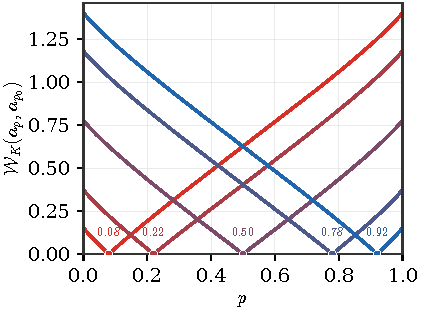
\includegraphics[width=.31\linewidth]{figures/discrete-markov-simplex-distances/sigma2-curves.pdf}
\hfill
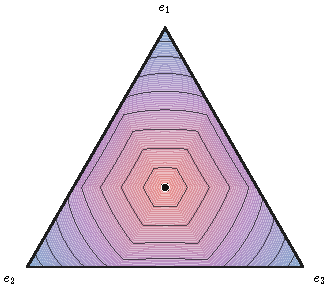
\includegraphics[width=.31\linewidth]{figures/discrete-markov-simplex-distances/sigma3-markov-levels.pdf}
\hfill
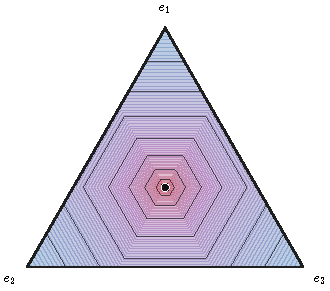
\includegraphics[width=.31\linewidth]{figures/discrete-markov-simplex-distances/sigma3-tv-levels.pdf}
\caption{\emph{Discrete Wasserstein distances on small Markov-chain simplices.} Left: the closed-form profiles \(r\mapsto \mathcal W_K(a_r,a_{r_0})\), with \(a_r=(r,1-r)\), for several anchors \(r_0\) on \(\Sigma_2\). Middle: numerical level sets of \(\mathcal W_K(a,\bar a)\) on \(\Sigma_3\), where \(\bar a=(1/3,1/3,1/3)\), computed from the local Riemannian norm induced by the complete-neighbor Markov chain. Right: the corresponding level sets for the ordinary \(W_2\) distance with \(d(i,j)=1\) for \(i\neq j\), i.e. \(W_2^2(a,\bar a)=\norm{a-\bar a}_{\mathrm{TV}}\).}
\label{fig:discrete-markov-simplex-distances}
\end{figure}

\subsection{Dynamic Unbalanced Wasserstein Distances}
\index{dynamic!unbalanced OT}% strictindex
\index{unbalanced OT}% strictindex
\label{sec-unbalanced-ot}

Balanced dynamic distances keep the total mass fixed: their tangent vectors are transport velocities or fluxes satisfying a continuity equation. Unbalanced distances use a different tangent model. A tangent vector now has both a spatial component and a reaction component, so mass can move, disappear and reappear. This subsection isolates this reaction--transport geometry before its use for gradient flows in Section~\ref{sec-dynamic-unbalanced-wfr-flows}.
\index{reaction-transport geometry}% strictindex
\index{tangent space!unbalanced}% strictindex

\paragraph{Balance equation and tangent variables.}
Unbalanced dynamic transport is obtained by allowing mass to be created and destroyed along the path. The continuity equation is replaced by a balance equation, and an admissible tangent direction is a pair \((m,s)\): the flux \(m\) transports mass in space, while the source \(s\) changes the amount of mass locally. This dynamic formulation underlies the Hellinger--Kantorovich and Wasserstein--Fisher--Rao metrics~\cite{LieroMielkeSavareShort,2017-chizat-focm}; its equivalence with static entropy-transport and cone formulations is developed in~\cite{LieroMielkeSavareLong,2015-chizat-unbalanced}. A representative quadratic balance equation is
\index{balance equation}% strictindex
\index{continuity equation}% strictindex
\index{growth term}% strictindex
\index{source term}% strictindex
	\[
		\partial_t\rho_t+\nabla\!\cdot m_t=s_t,
		\qquad
		\int_0^1\!\int
		\left(\frac{|m_t|^2}{\rho_t}+\kappa^2\frac{s_t^2}{\rho_t}\right)\d x\,\d t,
	\]
	with the usual perspective convention: zero flux and zero source through zero density cost nothing, whereas nonzero flux or source through zero density has infinite cost.

\paragraph{Reaction--transport action.}
The action attaches one price to displacement and another to local growth. This is the same notation as for balanced dynamic distances, except that the pointwise action now has three variables. On the velocity side, for a mass density \(a\geq 0\), a velocity \(w\in\RR^d\), and a relative growth rate \(g\in\RR\), define
	\begin{equation}
		A_\kappa(a,w,g)
		\eqdef
		a\bigl(\norm{w}^2+\kappa^2 g^2\bigr).
		\label{eq-wfr-velocity-action}
	\end{equation}
Thus, writing \(m_t=\rho_t v_t\) and \(s_t=\rho_t g_t\), the smooth action is \(\int_0^1\int A_\kappa(\rho_t,v_t,g_t)\d x\,\d t\) under \(\partial_t\rho_t+\nabla\!\cdot(\rho_t v_t)=g_t\rho_t\). The parameter \(\kappa\) fixes the relative cost of reaction and transport; changing it rescales the radial/angular balance in the associated cone metric.

For the convex measure formulation, one passes to the flux and source variables \(m=a w\) and \(r=a g\). The corresponding three-variable perspective is
	\begin{equation}
		J_\kappa(a,m,r)
		\eqdef
		\begin{cases}
			\displaystyle\frac{\norm{m}^2+\kappa^2 r^2}{a},
				& a>0,\\[6pt]
			0, & a=0,\ m=0,\ r=0,\\
			+\infty, & a=0,\ (m,r)\neq(0,0).
		\end{cases}
		\label{eq-wfr-momentum-perspective}
	\end{equation}
Equivalently, \(J_\kappa(a,m,r)=A_\kappa(a,m/a,r/a)\) when \(a>0\). For measure-valued triples, write \(\alpha\) for the transported measure, \(\omega\) for the vector-valued flux measure, and \(\sigma\) for the signed source measure. If \(\lambda\) dominates \(\alpha\), \(|\omega|\), and \(|\sigma|\), define
	\begin{equation}
		\mathbb J_\kappa(\alpha,\omega,\sigma)
		\eqdef
		\int
		J_\kappa\!\left(
			\frac{\d\alpha}{\d\lambda},
			\frac{\d \omega}{\d\lambda},
			\frac{\d \sigma}{\d\lambda}
		\right)\d\lambda .
		\label{eq-wfr-measure-action}
	\end{equation}
Since \(J_\kappa\) is convex and positively one-homogeneous in \((a,m,r)\), this definition is independent of the dominating measure \(\lambda\). Finite action forces both the flux and source to be absolutely continuous with respect to the transported mass.
\index{balance equation}% strictindex
\index{Hellinger-Kantorovich}% strictindex
\index{Wasserstein-Fisher-Rao}% strictindex

\paragraph{Static and dynamic viewpoints.}
The dynamic balance-equation formula is not a separate object from static unbalanced OT: it is the least-action representation of the same cone distance. The next proposition records this identification and fixes the normalization used later.

\begin{prop}[Static/dynamic equivalence for unbalanced OT]\label{prop-static-dynamic-unbalanced}
\index{static-dynamic equivalence}% strictindex
\index{unbalanced OT}% strictindex
		Fix the action above and let $\CW_\kappa$ be the corresponding static cone value, with the cone metric normalized to the same growth scale $\kappa$. For nonnegative finite measures $\alpha_0,\alpha_1$ on $\RR^d$, the dynamic value
	\begin{equation}\label{eq-dynamic-unbalanced-ot}
		\WFR_\kappa^2(\alpha_0,\alpha_1)
		\eqdef
		\inf_{\substack{\partial_t\alpha_t+\nabla\cdot \omega_t=\sigma_t\\
		\alpha_{t=0}=\alpha_0,\ \alpha_{t=1}=\alpha_1}}
		\int_0^1
		\mathbb J_\kappa(\alpha_t,\omega_t,\sigma_t)\,\d t
	\end{equation}
		equals the static cone formulation $\CW_\kappa(\alpha_0,\alpha_1)$. Hence the static unbalanced problem and the balance-equation least-action problem define the same geodesic distance.
\end{prop}

\begin{proof}
	The cone construction turns variation of mass into radial motion and spatial transport into angular motion on $\mathfrak C[\RR^d]$. Applying the Benamou--Brenier theorem on the cone to the lifted endpoint measures gives a dynamic least-action problem on $\mathfrak C[\RR^d]$ whose static value is the cone value $\CW_\kappa$. This is the standard static/dynamic identification for the Hellinger--Kantorovich and Wasserstein--Fisher--Rao metrics~\cite{LieroMielkeSavareShort,LieroMielkeSavareLong,2017-chizat-focm,2015-chizat-unbalanced}.
\index{cone!lifting}% strictindex
\index{Benamou-Brenier}% strictindex

	Projecting a cone curve back to the base space with the squared cone radius as weight produces a measure curve \(\alpha_t\), a spatial flux measure \(\omega_t\), and a source measure \(\sigma_t\) satisfying the balance equation. With the matching normalization of the cone metric, the cone kinetic energy decomposes exactly into the three-variable perspective action \(\mathbb J_\kappa\) in~\eqref{eq-dynamic-unbalanced-ot}. Conversely, any finite-action triple \((\alpha_t,\omega_t,\sigma_t)\) can be lifted to a cone curve whose radial velocity realizes the growth term and whose spatial velocity realizes the transport term, with the same action after relaxation. The two infima are therefore equal; lower semicontinuity gives the general finite-measure statement from the smooth positive case.
\index{balance equation}% strictindex
\index{lower semicontinuity}% strictindex
\end{proof}

\paragraph{Balanced versus unbalanced geodesics.}
The distinction is visible already for one-dimensional mixtures with mismatched modal masses. Balanced transport must physically move the excess mass, whereas unbalanced transport can trade transport against reaction.

\begin{figure}[H]
\centering
\setlength{\tabcolsep}{1pt}
\begin{tabular}{@{}rccccc@{}}
& \small $t=0$ & \small $t=.25$ & \small $t=.5$ & \small $t=.75$ & \small $t=1$ \\
\small balanced &
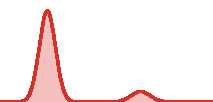
\includegraphics[width=.165\linewidth]{figures/dynamic-unbalanced-geodesic/balanced-t000.pdf} &
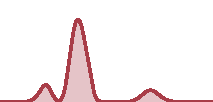
\includegraphics[width=.165\linewidth]{figures/dynamic-unbalanced-geodesic/balanced-t025.pdf} &
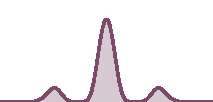
\includegraphics[width=.165\linewidth]{figures/dynamic-unbalanced-geodesic/balanced-t050.pdf} &
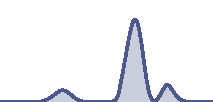
\includegraphics[width=.165\linewidth]{figures/dynamic-unbalanced-geodesic/balanced-t075.pdf} &
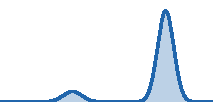
\includegraphics[width=.165\linewidth]{figures/dynamic-unbalanced-geodesic/balanced-t100.pdf} \\
\small unbalanced &
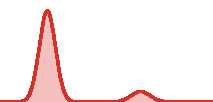
\includegraphics[width=.165\linewidth]{figures/dynamic-unbalanced-geodesic/unbalanced-t000.pdf} &
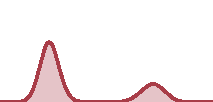
\includegraphics[width=.165\linewidth]{figures/dynamic-unbalanced-geodesic/unbalanced-t025.pdf} &
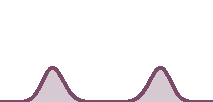
\includegraphics[width=.165\linewidth]{figures/dynamic-unbalanced-geodesic/unbalanced-t050.pdf} &
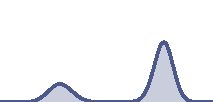
\includegraphics[width=.165\linewidth]{figures/dynamic-unbalanced-geodesic/unbalanced-t075.pdf} &
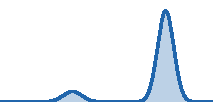
\includegraphics[width=.165\linewidth]{figures/dynamic-unbalanced-geodesic/unbalanced-t100.pdf}
\end{tabular}
\caption{\emph{Balanced and unbalanced Sinkhorn-barycenter interpolations between two one-dimensional Gaussian mixtures with swapped modal masses.} The balanced row conserves total mass, so excess mass from the dominant left mode must move along the line toward the dominant right target mode, producing transient mass in the middle. The unbalanced row uses KL-relaxed marginal constraints; mass can be attenuated near overrepresented modes and recreated near underrepresented modes, giving a reaction--transport interpolation closer to the Wasserstein--Fisher--Rao intuition.}
\index{Sinkhorn!barycenter}% strictindex
\index{unbalanced!barycenter}% strictindex
\label{fig:dynamic-unbalanced-geodesic}
\end{figure}
